\newpage
\section{Ergebnisse}
\label{sec:Ergebnisse}
In diesem Kapitel werden die zentralen Ergebnisse der Arbeit präsentiert.
Im Mittelpunkt steht der entwickelte \acs{aas}-Demonstrator, der die prototypische Umsetzung des digitalen Zwillings des Abfüll- und Verschließmoduls der robocell-Linie zeigt.
Darauf folgt die Analyse des eingesetzten Autoencoder-Modells zur Anomalieerkennung sowie die Vorstellung der beiden Anwendungsfälle \acs{dpp} und automatisierte Generierung der \acs{aas}.
Abschließend werden die im Projekt eingesetzten Softwarelösungen und Tools evaluiert.

\subsection{AAS-Demonstrator für die robocell}
\label{sec:AAS-Demonstrator}
Der \acs{aas}-Demonstrator basiert auf dem standardisierten Konzept der \acs{aas}.
Als zentrale Laufzeitumgebung kommt die Eclipse BaSyx-Plattform zum Einsatz, während für die Datenanbindung standardisierte Protokolle wie OPC~UA sowie HTTP/REST verwendet werden.
Der Demonstrator umfasst neben der Haupt-AAS der robocell-Maschine auch exemplarische AAS untergeordneter Komponenten, wodurch eine modulare und hierarchisch aufgebaute digitale Repräsentation entsteht.

Im weiteren Verlauf wird zunächst die Architektur des Gesamtsystems vorgestellt.
Sie dient der Verwaltung und Bereitstellung aller modellierten \acs{aas} und bildet die Grundlage für die dynamische Erweiterung um Echtzeit- und Zeitreihendaten.
Anschließend werden die im Demonstrator abgebildeten Aspekte der Maschine beschrieben, gegliedert in statische und dynamische Submodelle.
Den Abschluss bildet eine kurze Reflexion über zentrale Herausforderungen, die während der Implementierung aufgetreten sind.

\subsubsection{Systemarchitektur}

Die Architektur besteht aus mehreren Komponenten, die zusammen einen aktiven digitalen Zwilling im Sinne einer Typ-2-\acs{aas} ermöglichen.
Sie basiert auf containerisierten Diensten, die in einer gemeinsamen Docker-Umgebung verwaltet werden und über ein internes Netzwerk miteinander kommunizieren.
Der modulare Aufbau erleichtert Erweiterungen und Anpassungen und schafft so eine skalierbare Infrastruktur für unterschiedliche Anforderungen.

Als Laufzeitumgebung zur Bereitstellung und Verwaltung der \acs{aas} kommt Eclipse BaSyx zum Einsatz.
Der ursprünglich vorgesehene AASX Server Blazor wurde zugunsten von BaSyx ersetzt, da die Plattform mehr Flexibilität und zusätzliche Funktionen für die Umsetzung digitaler Zwillinge bietet.
Abbildung~\ref{fig:BaSyxArchitektur} zeigt den Aufbau des Systems, das als zentrales BaSyx-Backend für die Verwaltung aller \acs{aas}-Komponenten zuständig ist.

\newpage
\begin{figure}[htbp]
    \centering
        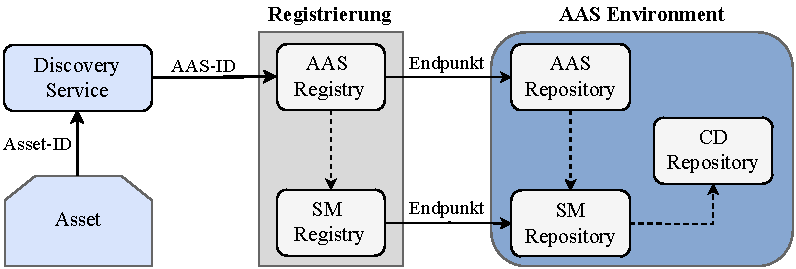
\includegraphics[width=1\textwidth]{Bilder/Ergebnisse/Systemarchitektur/BaSyx.pdf}
    \caption{Systemarchitektur BaSyx-Backend}
    \label{fig:BaSyxArchitektur}
\end{figure}

Der Discovery Service übernimmt die Auflösung einer Asset-\acs{id} (globalAssetId) in die zugehörige \acs{aas}-\acs{id} und ermöglicht so das gezielte Auffinden einer \acs{aas} im Gesamtsystem. 
Die Registries dienen als Verzeichnisse aller registrierten \acs{aas} und Submodelle einschließlich ihrer Endpunkte innerhalb der \acs{aas} Environment, wobei die \acs{aas} Registry optional auch Referenzen auf die Submodel Registry (SM Registry) enthalten kann. 

Die \acs{aas} Environment selbst beherbergt die eigentlichen Inhalte und ist in drei Repositories gegliedert. 
Das AAS Repository verwaltet die \acs{aas} einschließlich Asset-Metadaten und Referenzen auf Submodelle. 
Das Submodel Repository (SM Repository) speichert die Submodelle mit ihren jeweiligen Inhalten und Referenzen auf die zugehörigen Concept Descriptions. 
Diese werden im \acs{cd} Repository verwaltet und beinhalten alle semantischen Beschreibungen.

Alle Komponenten verfügen dabei über eine standardisierte REST-API, die sowohl anderen Systemen als auch den Komponenten selbst einen einheitlichen Zugriff auf ihre Inhalte ermöglicht. 
Zudem sind sie an eine gemeinsame MongoDB angebunden, in der sämtliche Daten persistent gespeichert werden.

Die dynamische Erweiterung ergänzt die Kernarchitektur um die Fähigkeit zur Verarbeitung von Echtzeit- und Zeitreihendaten. 
Abbildung~\ref{fig:DynamischeErweiterungArchitektur} zeigt den Aufbau der zusätzlichen Komponenten sowie deren Zusammenspiel mit dem bestehenden System.

Der Datengenerator und der Maschinensimulator simulieren das Abfüll- und Verschließmodul und erzeugen sowohl Zustands- als auch Prozessdaten. 
Beide Anwendungen stellen ihre Daten über einen \acs{opcua} Server bereit und sind über die Databridge direkt an die AAS Environment im BaSyx-Backend angebunden.
Zusätzlich werden die vom Datengenerator simulierten Werte mithilfe von Telegraf kontinuierlich in eine InfluxDB geschrieben, wodurch eine historische Datenbasis entsteht. 

% \begin{figure}[htbp]
%     \centering
%         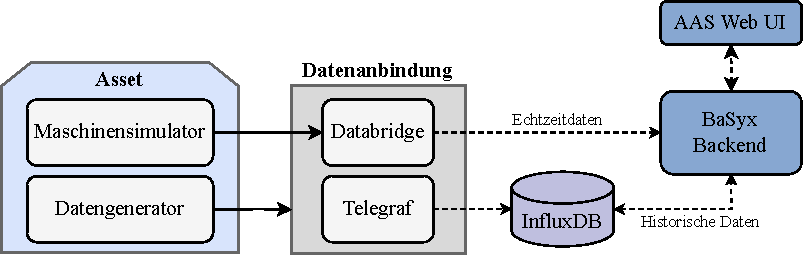
\includegraphics[width=1\textwidth]{Bilder/Ergebnisse/Systemarchitektur/DynamischeErwweiterung.pdf}
%     \caption{Dynamische Erweiterung der BaSyx-Architektur}
%     \label{fig:DynamischeErweiterungArchitektur}
% \end{figure}

\newpage
\begin{figure}[htbp]
    \centering
        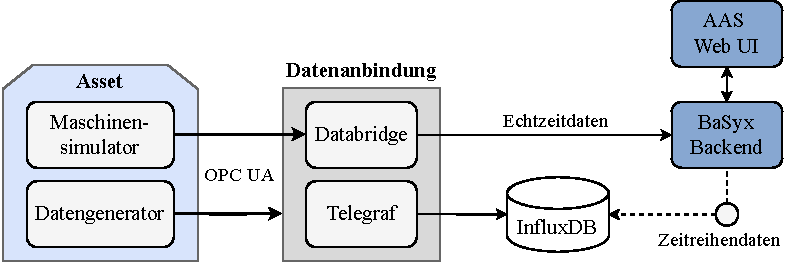
\includegraphics[width=1\textwidth]{Bilder/Ergebnisse/Systemarchitektur/DynamischeErwweiterungNeu.pdf}
    \caption{Erweiterung der BaSyx-Architektur}
    \label{fig:DynamischeErweiterungArchitektur}
\end{figure}

% \vspace{-0.5em}
Zur Weiterverarbeitung und Visualisierung, sowohl der statischen Inhalte der AAS als auch der durch die dynamische Erweiterung ergänzten Echtzeit- und Zeitreihendaten, kommt die AAS Web UI zum Einsatz. 
Alternativ könnten auch benutzerdefinierte Anwendungen verwendet werden, die beispielsweise zusätzliche Analysen ermöglichen oder spezifische Anforderungen erfüllen.

Die AAS Web UI greift über die standardisierten Schnittstellen der Komponenten des zuvor vorgestellten BaSyx-Backends auf die Registrierungsdaten der AAS sowie deren Submodelle und Inhalte zu. 
Statische Daten und Echtzeitdaten werden dabei direkt aus dem Submodel Repository abgefragt. 
Bei Zeitreihendaten hingegen ist nicht der eigentliche Dateninhalt in der AAS gespeichert, sondern lediglich ein Verweis auf den Endpunkt der InfluxDB hinterlegt. 
Die AAS Web UI nutzt diesen Endpunkt, um die historischen Daten direkt aus der Datenbank abzurufen und in der Web-Oberfläche zu visualisieren.

\subsubsection{Statische Submodelle}
Die statische Modellierung des Demonstrators erfolgte ausschließlich im Package Explorer.
Dazu wurden alle relevanten AAS sowie die zugehörigen Submodelle angelegt, mit Inhalten befüllt, semantisch angereichert und mit eindeutigen Identifikatoren versehen.
Als Hauptdatenquellen dienten die technischen Dokumentationen der robocell, insbesondere die Betriebsanleitung, sowie Informationen aus dem PLM-System Agile.

Abbildung~\ref{fig:PackageExplorerRobocell} zeigt die Gesamtübersicht des Abfüll- und Verschließmoduls. 
Die statischen Submodelle sind darin mit einer Nummer gekennzeichnet, die der im Folgenden verwendeten Gliederung entspricht. 
Sie beinhalten feststehende, beschreibende Inhalte, die nicht zur Laufzeit geändert werden. 
Zur besseren Veranschaulichung wird das Submodell BOM ausführlicher beschrieben.
Die grundlegende Struktur der weiteren statischen Submodelle ist im Anhang~\ref{sec:AnhangStatischeSubmodelle} ergänzend anhand von Screenshots dokumentiert.

\begin{figure}[htbp]
    \centering
        \includegraphics[width=1\textwidth]{Bilder/ErgebnissePackageExplorer/AASrobocellTestAuflösung.PNG}
    \caption{\acs{aas} des Abfüll- und Verschließmoduls}
    \label{fig:PackageExplorerRobocell}
\end{figure}

\subsubsection*{1) Typenschild}
\vspace{-0.5em} 
Das Submodell Typenschild bildet die zentrale Identifikationsstelle der Maschine innerhalb der AAS. 
Es erfasst grundlegende Angaben wie Hersteller, Seriennummer, Produkttyp oder Softwareversionen. 
Funktional entspricht es einem physischen Typenschild, erweitert dieses jedoch um maschinenlesbare und interoperable Inhalte. 
Darüber hinaus bietet es den Vorteil, dass auch zusätzliche Dateien wie Zertifikate oder Logos direkt eingebunden werden können.

\subsubsection*{2) Technische Daten}
\vspace{-0.5em}

Das Submodell Technische Daten dient als technisches Datenblatt der Maschine.  
Es gliedert sich in die Bereiche Allgemeine Informationen sowie Technische Eigenschaften. 
Letztere sind in mehreren \acsp{smc} organisiert, beispielsweise für Produktionsmedien, Umgebungsbedingungen, elektrische Daten oder den Verarbeitungsbereich. 
Die einzelnen \acsp{smc} enthalten überwiegend Properties oder Ranges, die Parameter, beispielsweise elektrische Kenndaten, beschreiben.
Auf diese Weise sind alle relevanten technischen Angaben an einem zentralen Ort gebündelt, was der redundanten Pflege in verschiedenen Systemen oder Dokumenten entgegenwirkt. 

\subsubsection*{3) BOM}
\vspace{-0.5em}

Das Submodell \acs{bom} dient dazu, die Maschinenstruktur sichtbar zu machen und die Beziehungen zwischen ihren einzelnen Komponenten hierarchisch abzubilden, vergleichbar mit einer digitalen Stückliste.
Dabei enthält es verschiedene Entitäten, die jeweils eine untergeordnete Komponente repräsentieren.
Die Beziehungen zwischen den Komponenten werden über Relationship-Elemente mit einer eindeutigen semanticId gemäß dem \acs{smt} Hierarchical Structures Enabling Bills of Material \cite{SpezifikationHierachischeStrukturen} hergestellt.

Zur Veranschaulichung wurde die Grundmaschine als Beispiel gewählt, da sie weniger komplex als die Maschinenebene ist, aber dennoch alle relevanten Strukturelemente enthält.
Abbildung~\ref{fig:BOMSubmodelGrundmashcine} zeigt das entsprechende Submodell, in dem weitere untergeordnete Komponenten aufgeführt sind, darunter auch das Bedientableau.
Dieses ist als Self-Managed Entity angelegt und über die globalAssetId mit seiner AAS verknüpft (Abbildung~\ref{fig:AASBedientableau}), die wiederum ein eigenes BOM-Submodell mit weiteren Unterkomponenten enthält.

\begin{figure}[htbp]
    \centering
        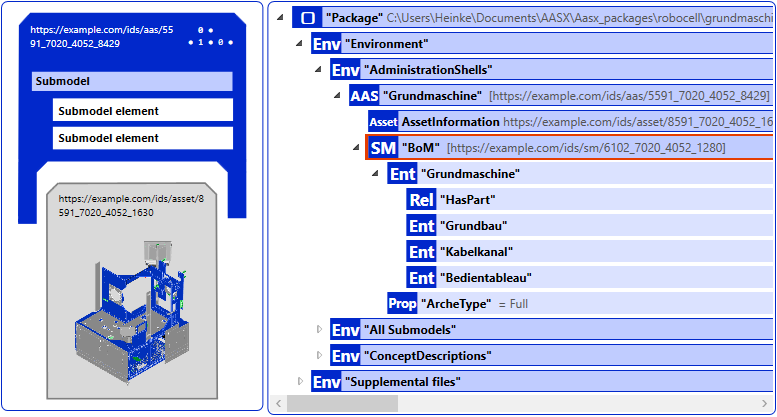
\includegraphics[width=1\textwidth]{Bilder/ErgebnissePackageExplorer/AASGrundmaschine.PNG}
    \caption{Submodell \acs{bom} der Grundmaschine}
    \label{fig:BOMSubmodelGrundmashcine}
\end{figure}

\begin{figure}[htbp]
    \centering
        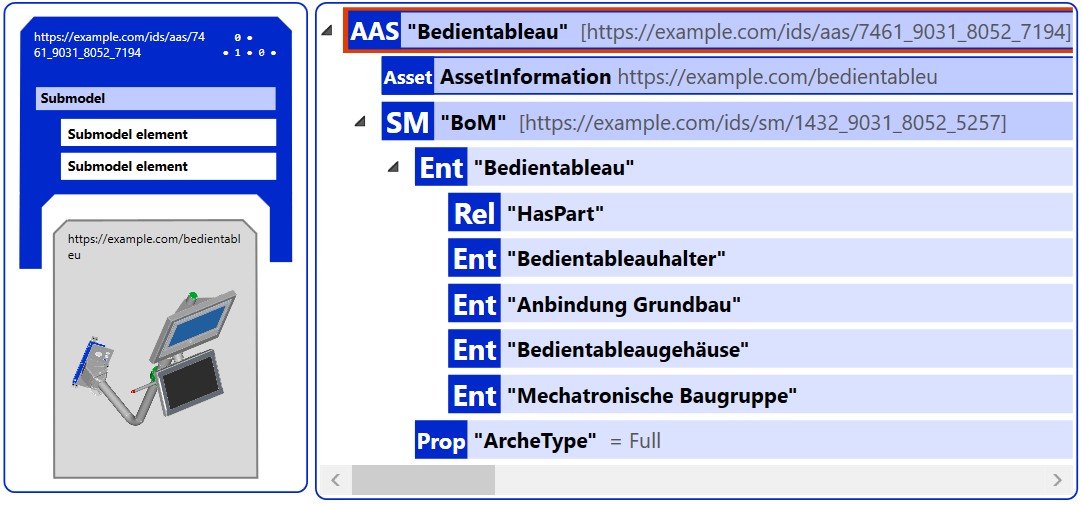
\includegraphics[width=1\textwidth]{Bilder/ErgebnissePackageExplorer/BedientableauTest.PNG}
    \caption{\acs{aas} des Bedientableaus}
    \label{fig:AASBedientableau}
\end{figure}


Mit diesem Prinzip lässt sich die gesamte Maschine rekursiv abbilden. 
Jede Komponente wird als eigenständige AAS geführt und ist somit unabhängig von der übergeordneten Struktur wiederverwendbar. 
Dies ermöglicht eine modulare und herstellerübergreifende Integration, da auch externe Komponenten eingebunden werden können.

\subsubsection*{4), 5) Dokumentation und 3D-Modelle}
\vspace{-0.5em}

Beide Submodelle dienen der Bereitstellung und Klassifizierung zentraler Maschinendateien. 
Das Submodell Dokumentation umfasst technische Unterlagen wie%
\pagebreak
~die Betriebsanleitung oder die Netzwerkübersicht, während das Submodell 3D-Modelle CAD-Daten zur Geometrie beinhaltet. 
Alle Dateien sind als File-Elemente direkt in die Struktur der AAS eingebettet und jeweils in eigenen \acsp{smc} organisiert, die zusätzlich Metainformationen zu Identifikation, Klassifikation und Versionierung enthalten. 
Das Submodell 3D-Modelle könnte darüber hinaus um weitere Metadaten, etwa zu Darstellungsoptionen oder Geometrieinformationen, ergänzt werden, was im Demonstrator jedoch nicht umgesetzt wurde. 
Dadurch ermöglichen beide Submodelle nicht nur das Einbetten von Dateien, sondern auch deren eindeutige Beschreibung und Rückverfolgbarkeit über den gesamten Lebenszyklus hinweg.

\subsubsection*{6) Wartung}
\vspace{-0.5em}

Das Submodell Wartung bildet den digitalen Wartungsplan der Maschine ab. 
Für jede wartungsrelevante Komponente sind in eigenen \acsp{smc} letzte Wartungszeitpunkte, Intervalle, zuständige Personen oder Organisationen sowie die vorgesehenen Maßnahmen hinterlegt. 
Es ermöglicht damit die strukturierte Verwaltung sowohl bereits durchgeführter als auch anstehender Wartungen und gewährleistet eine nachvollziehbare Dokumentation. 
Darüber hinaus schafft das Submodell die Grundlage für eine dynamische Erweiterung. 
So könnte beispielsweise ein Betriebsstundenzähler angebunden werden, der automatisch Wartungsbedarf erkennt, oder es könnte in Kombination mit \acs{pm}-Ansätzen genutzt werden, um auf Basis von Sensordaten proaktiv Wartungsmaßnahmen abzuleiten und diese direkt in der AAS darzustellen. 

\subsubsection*{Zusammenfassung}
\vspace{-0.5em}

Die statischen Submodelle verdeutlichen, wie zentrale Stammdaten einer Maschine strukturiert und standardisiert in der \acs{aas} gebündelt werden können. 
Dadurch wird eine einfache Weitergabe der Informationen entlang der Wertschöpfungskette ermöglicht. 
Die \acs{aas} lässt sich beispielsweise in Form einer AASX-Datei an einen Betreiber übergeben, der direkten Zugriff auf die Daten benötigt.
Zugleich erlaubt die rekursive Einbindung von Komponenten-\acs{aas} die nahtlose Integration in den digitalen Zwilling der Gesamtmaschine. 

Durch die Orientierung an standardisierten \acsp{smt} und die Nutzung von Concept Descriptions zur semantischen Beschreibung können die Inhalte dabei von unterschiedlichen Systemen oder Personen gleichermaßen interpretiert und genutzt werden. 
Auf diese Weise wird nicht nur die Interoperabilität gewährleistet, sondern auch die Rückverfolgbarkeit von Maschinendaten über den gesamten Lebenszyklus gestärkt.

\newpage
\subsubsection{Dynamische Submodelle}
\label{sec:DynamischeSubmodelle}
Neben den statischen Submodellen wurden im Demonstrator auch dynamische Submodelle umgesetzt.
Sie ermöglichen die kontinuierliche Erfassung und Aktualisierung von Maschinen- und Prozessdaten sowie die Interaktion mit dem zugrunde liegenden Asset.
Da im Rahmen dieser Arbeit keine reale Maschine zur Verfügung stand, wird dieses Asset durch den Datengenerator und den Maschinensimulator repräsentiert.

Die technische Umsetzung und die zugrunde liegenden Datenflüsse orientieren sich an etablierten Industriearchitekturen, sodass die Schnittstellen und Funktionsweisen ohne Anpassungen auch mit einem realen System genutzt werden könnten.
Durch diese Erweiterung erfüllt der Demonstrator die Anforderungen an einen digitalen Zwilling gemäß der in Kapitel~\ref{sec: DT} beschriebenen Klassifizierung.

\subsubsection*{Prozessdaten}
\vspace{-0.5em}
Das Submodell Prozessdaten erfasst die Prozessgrößen Füllstand, Durchfluss, Anzahl abgefüllter Einheiten und Druck.
Die Werte stammen aus dem \acs{opcua} Server des Datengenerators, werden dort im Sekundentakt aktualisiert und über die Databridge nahezu in Echtzeit an die \acs{aas} übertragen.
Innerhalb der Databridge erfolgt dabei eine zweistufige Transformation.
Mithilfe des Jackson-Transformers werden die Rohdaten zunächst in ein JSON-Objekt überführt und anschließend mit JSONata gefiltert, sodass nur die relevanten Messgrößen in die Properties des Submodells übernommen werden.

\begin{figure}[htbp]
    \centering
    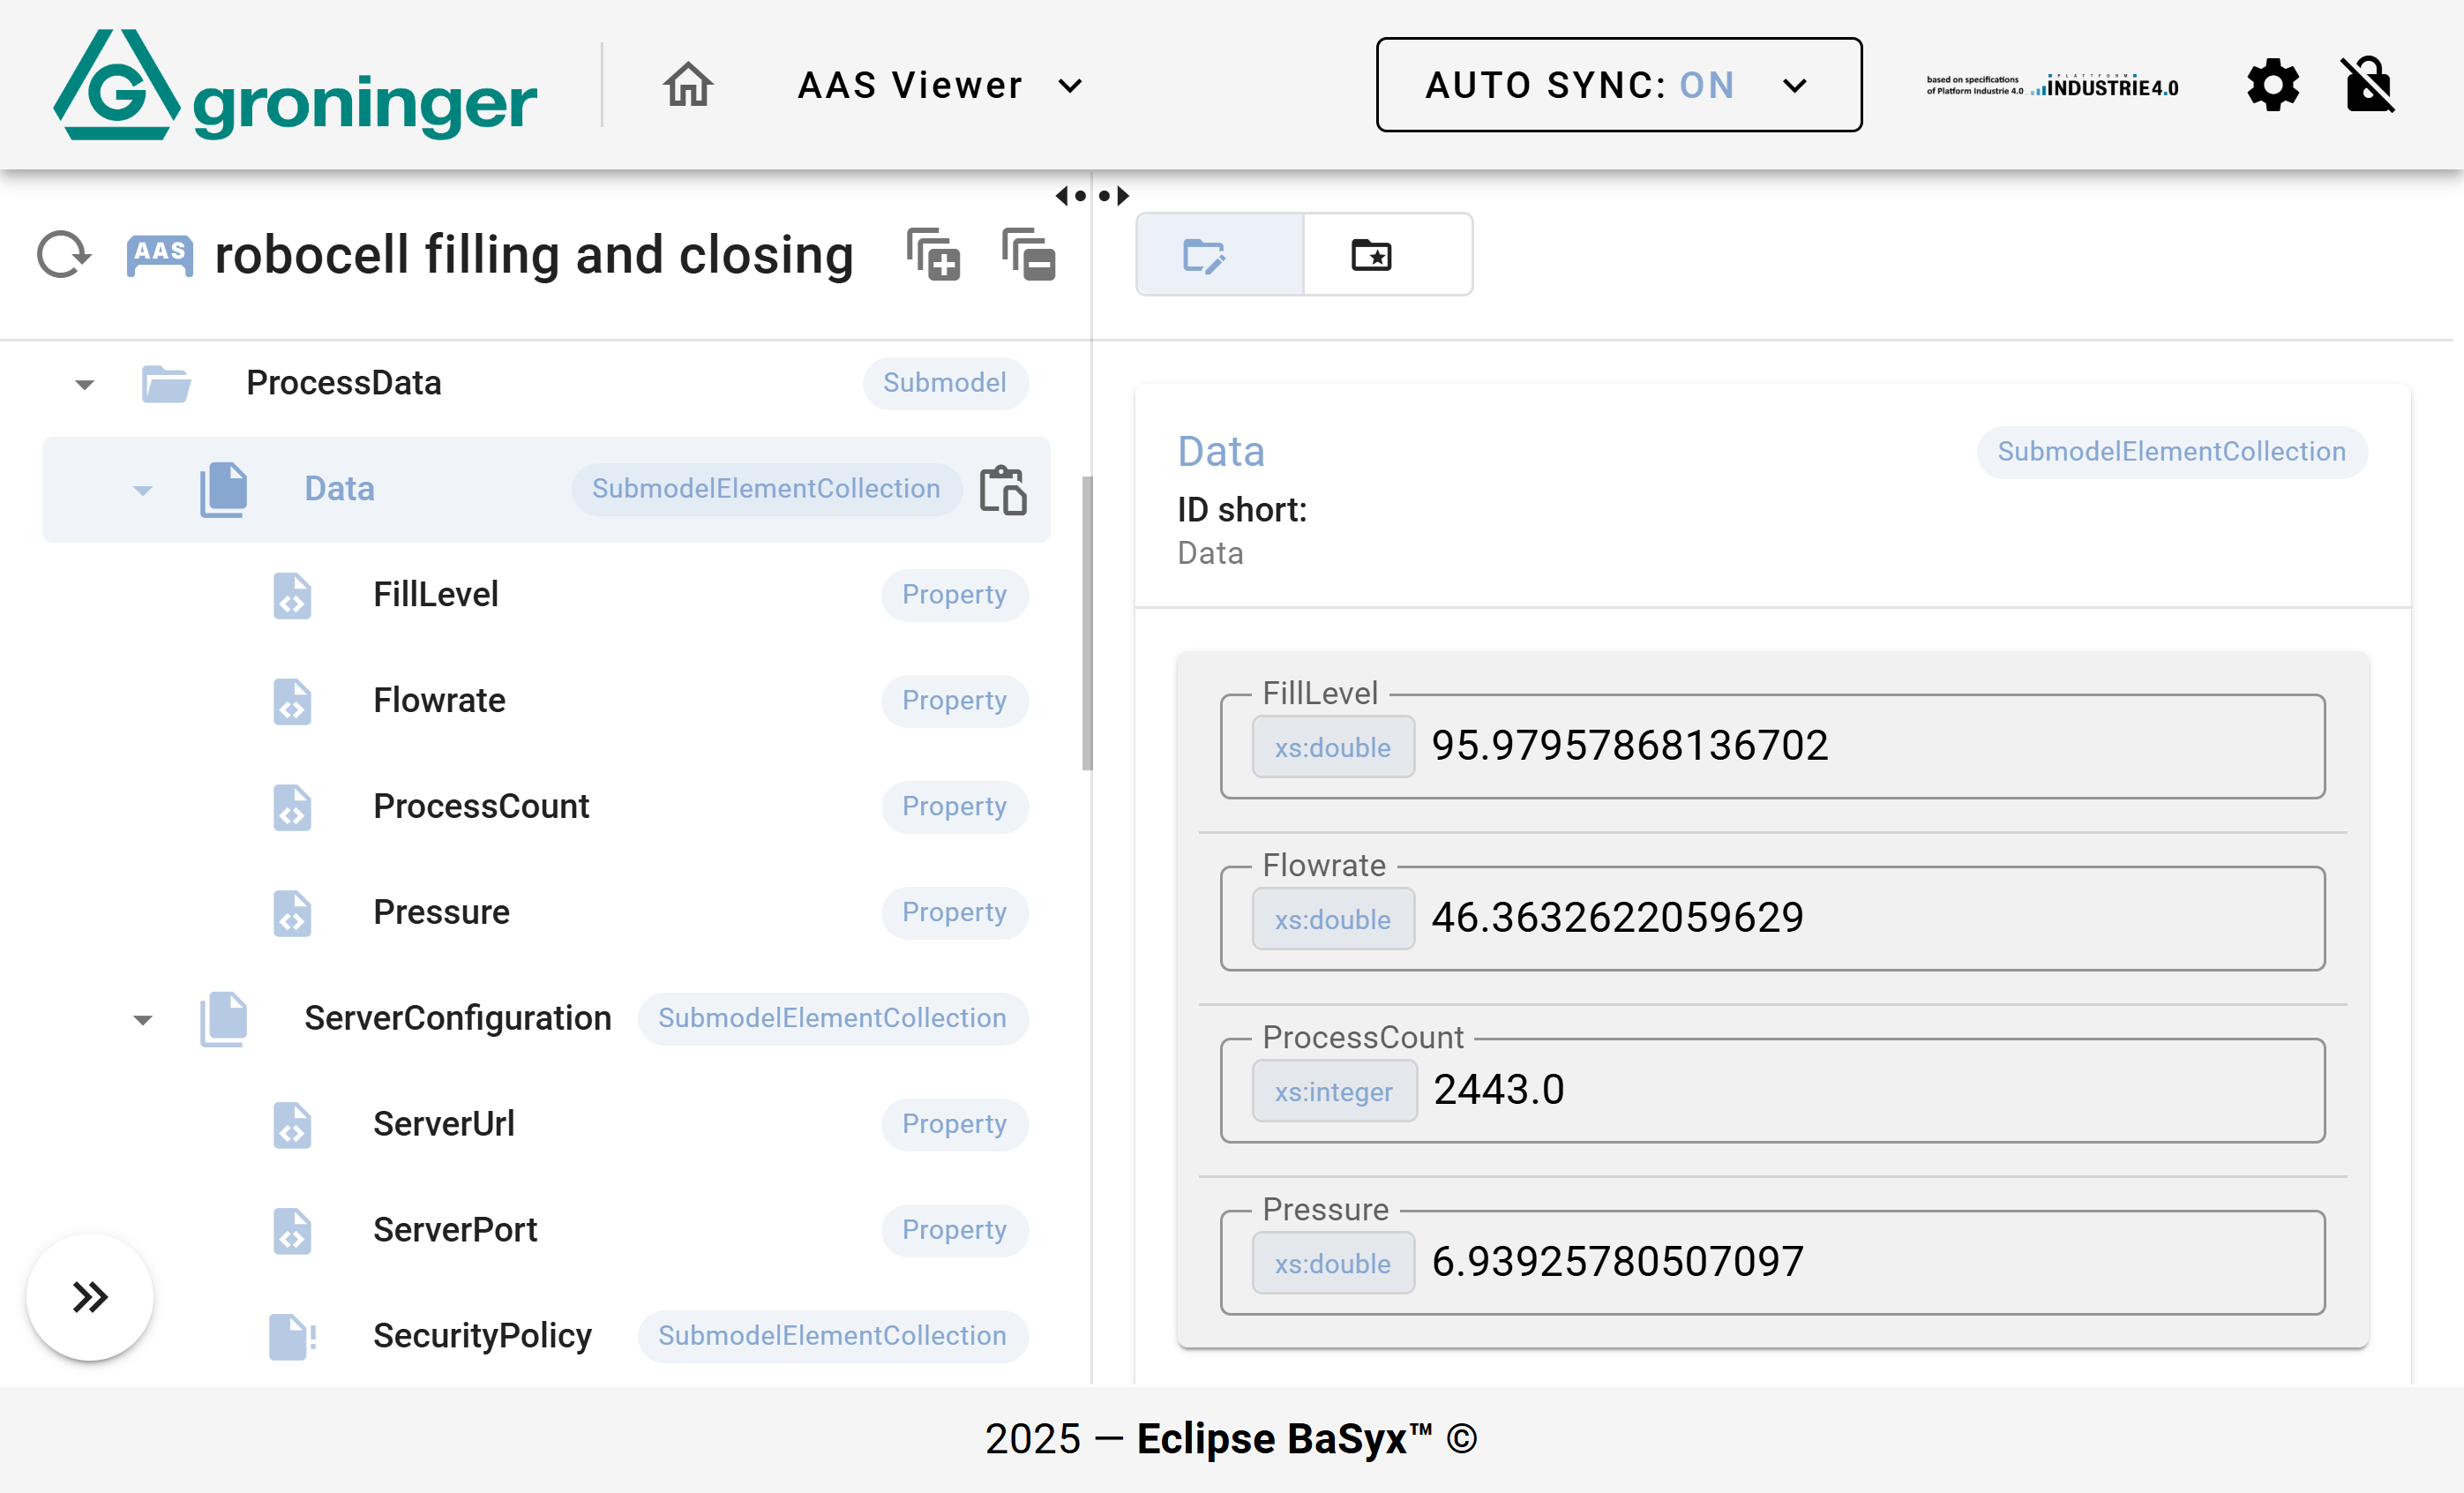
\includegraphics[width=1\textwidth]{Bilder/ErgebnisseAASWebUI/ProcessData.png}
    \caption{Visualisierung Submodell Prozessdaten}
    \label{fig:Processdata}
\end{figure}

Die Visualisierung der Prozessdaten erfolgt in der klassischen Elemente-Ansicht der AAS Web UI, wie in Abbildung~\ref{fig:Processdata} dargestellt, oder über ein speziell entwickeltes Plugin.
Damit die Werte in der Benutzeroberfläche aktuell bleiben, kann eine Synchronisationsfunktion aktiviert werden.
Dabei ruft die Weboberfläche die relevanten Daten in festen Intervallen, beispielsweise alle vier Sekunden, automatisch vom Repository ab.

Die Umsetzung ist protokolloffen und könnte grundsätzlich auf weitere Kommunikationsstandards wie \acs{mqtt} oder \acs{rest} erweitert werden.
Eine automatische bidirektionale Kommunikation, etwa das Zurückschreiben von Werten aus der \acs{aas} in externe Systeme, ist mit der eingesetzten Databridge derzeit jedoch nicht möglich.

\subsubsection*{Kontrollkomponente}
\vspace{-0.5em}
Das Submodell Kontrollkomponente dient der Abbildung und Visualisierung des aktuellen Maschinenstatus sowie der unterstützten Betriebsmodi.
Die Zustandsinformationen stammen aus dem Maschinensimulator, der sie in numerischer Form über einen \acs{opcua} Server bereitstellt.
Über die Databridge werden diese Werte in die \acs{aas} übertragen.
Vor der Speicherung erfolgt eine semantische Umwandlung mithilfe von JSONata, um die numerischen Codes in sprechende Zustandsbezeichnungen zu überführen.

Die Zustände orientieren sich am PackML-Standard (Packaging Machine Language), einem von der OMAC (Organization for Machine Automation and Control) entwickelten Modell zur einheitlichen Beschreibung von Maschinenzuständen und zulässigen Zustandsübergängen, insbesondere für Verpackungsmaschinen \cite{OMAC}. 
Der Standard definiert insgesamt 17 Maschinenzustände und legt fest, welche Übergänge zwischen diesen möglich sind. 
Dieses Konzept kommt auch bei der robocell-Linie zum Einsatz und ermöglicht eine konsistente und interoperable Erfassung des Maschinenstatus über verschiedene Systeme hinweg.

Die Visualisierung erfolgt über ein in die AAS Web UI integriertes Vue.js-Plugin, das den Maschinenstatus als PackML-Zustandsautomat darstellt.
Das Plugin basiert auf einer Entwicklung der Hochschule für Technik und Wirtschaft Berlin \cite{HTW1, HTW2} und wurde funktional angepasst, um es in die AAS Web UI zu integrieren und die im Demonstrator benötigten Steuer- und Anzeigeoptionen zu unterstützen.

Abbildung~\ref{fig:PackMLZustandsautomat} zeigt den Zustandsautomaten in der Benutzeroberfläche.
Damit Statusänderungen unmittelbar sichtbar werden, ist eine Polling-Logik implementiert, die den aktuellen Maschinenstatus in festen Intervallen aus dem Submodel Repository der AAS Environment abruft und im Zustandsautomaten aktualisiert.
Neben der reinen Statusanzeige erlaubt das Plugin auch die Steuerung zulässiger Zustandsübergänge direkt aus der Benutzeroberfläche heraus.
Befindet sich die Maschine beispielsweise im Zustand Execute, können Befehle wie Stop, Hold, Suspend oder Abort ausgelöst werden.
Darüber hinaus lässt sich der Betriebsmodus setzen, der ebenfalls als Property im Submodell verwaltet wird.

\begin{figure}[htbp]
    \centering 
    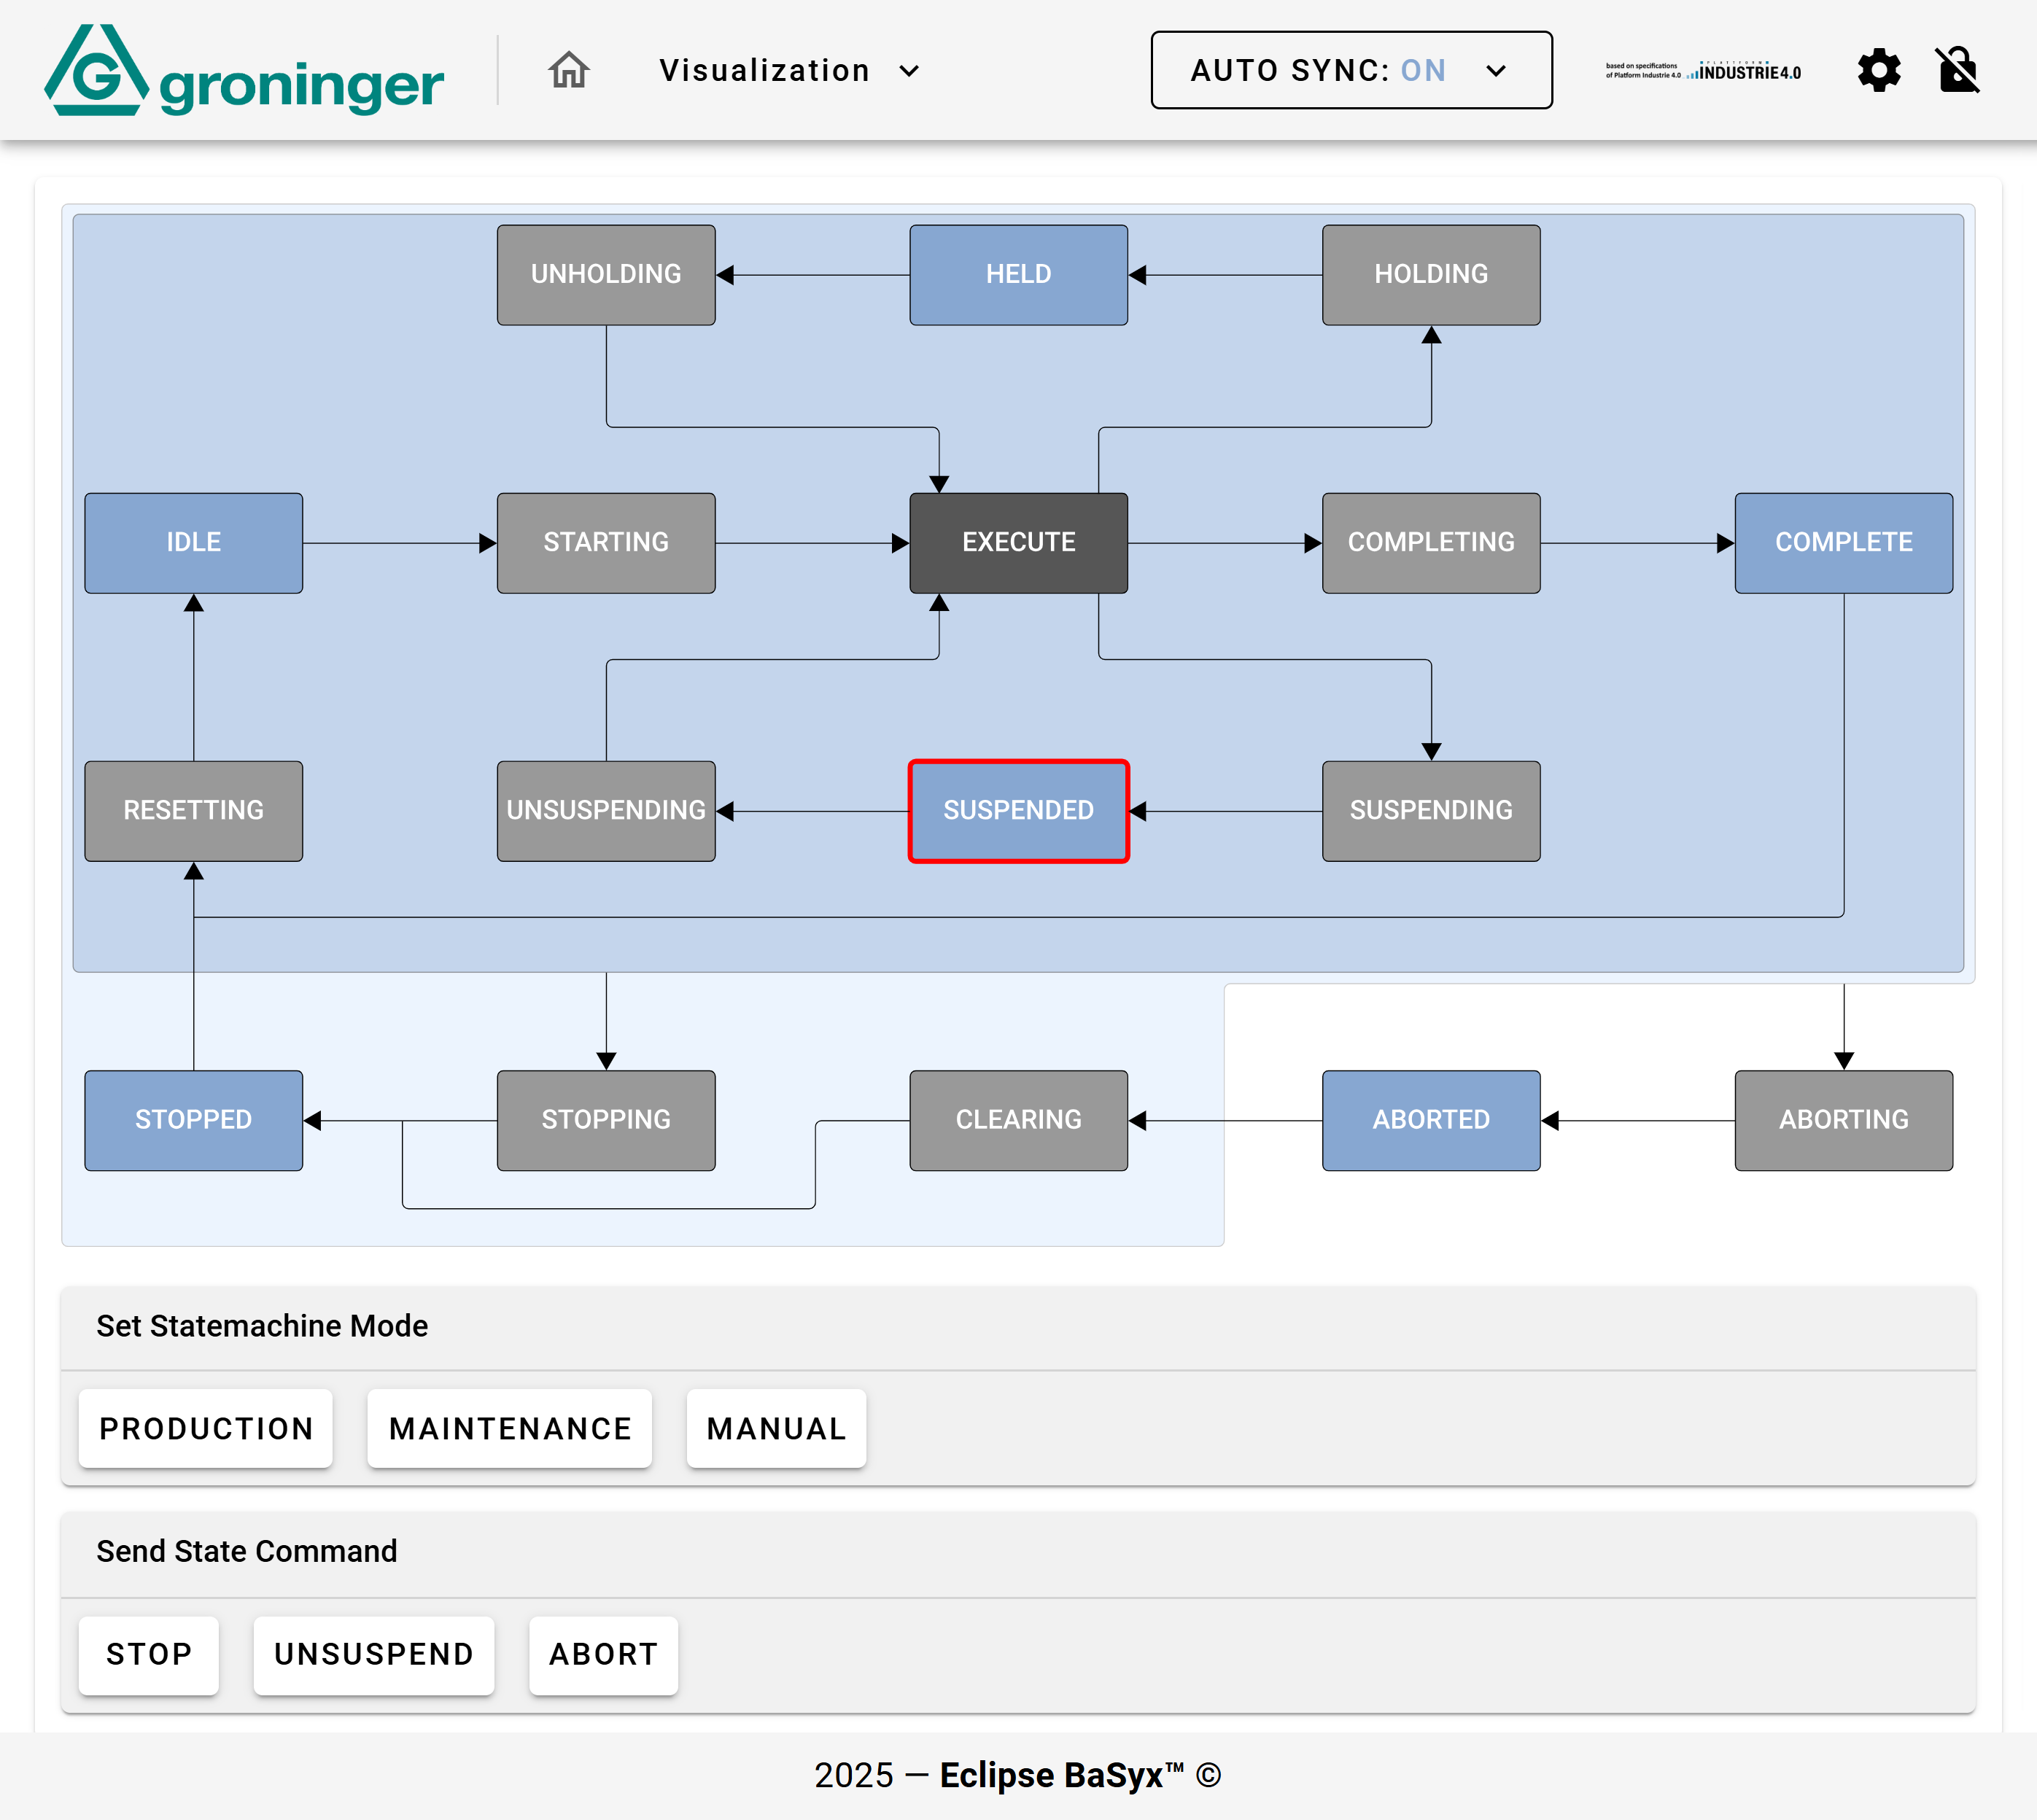
\includegraphics[width=1\textwidth]{Bilder/ErgebnisseAASWebUI/Kontrollkomponente.png} 
    \caption[Visualisierung Submodell Kontrollkomponente]{Visualisierung Submodell Kontrollkomponente (PackML-Zustandsautomat)} 
    \label{fig:PackMLZustandsautomat} 
\end{figure}
\vspace{-0.5em}

Neben der reinen Statusanzeige erlaubt das Plugin auch die Steuerung zulässiger Zustandsübergänge direkt aus der Benutzeroberfläche heraus.
Befindet sich die Maschine beispielsweise im Zustand Execute, können Befehle wie Stop, Hold, Suspend oder Abort ausgelöst werden.
Darüber hinaus lässt sich der Betriebsmodus (Produktion, Manuell oder Wartung) setzen, der ebenfalls als Property im Submodell verwaltet wird.


Im Demonstrator werden Befehle direkt per WebSocket an den Maschinensimulator übermittelt und dort ohne weitere Prüfungen übernommen. 
Dadurch entsteht eine direkte Feedback-Schleife zwischen der \acs{aas} und dem simulierten Asset.
In einer realen Maschine würden diese Signale hingegen zunächst über ein geeignetes Industrieprotokoll wie \acs{opcua} an die speicherprogrammierbare Steuerung (SPS) übertragen und dort validiert werden müssen, bevor der neue Zustand an die \acs{aas} zurückgemeldet wird.

\subsubsection*{Zeitreihendaten}
\vspace{-0.5em}

Das Submodell Zeitreihendaten dient der Einbettung historischer Messwerte in die AAS.
Im Demonstrator werden exemplarisch die Messgrößen Druck und Temperatur genutzt, die vom \acs{opcua} Server des Datengenerators bereitgestellt und mithilfe von Telegraf fortlaufend in der InfluxDB gespeichert werden.

Die Anbindung an die \acs{aas} erfolgt über ein LinkedSegment (eine \acs{smc}) im Submodell, das alle für die Datenabfrage erforderlichen Parameter enthält, wie den Endpunkt der InfluxDB und die zugehörige Abfragebeschreibung. 
Dadurch können Anwendungen, die auf die \acs{aas} zugreifen, die Zeitreihendaten gezielt abrufen, ohne Details zur technischen Implementierung der Datenbank kennen zu müssen.

Zur Visualisierung steht in der AAS Web UI ein Plugin bereit, das die im LinkedSegment hinterlegten Parameter nutzt, um Abfragen an die InfluxDB zu stellen.
Ein Nutzer kann dabei auswählen, ob einzelne Messgrößen oder kombinierte Ansichten mehrerer Werte angezeigt werden sollen. 
Abbildung~\ref{fig:LiniendiagrammBaSyx} zeigt exemplarisch ein Liniendiagramm mit den zeitlichen Verläufen von Druck und Temperatur über einen Zeitraum von fünf Minuten.

\begin{figure}[htbp]
    \centering
        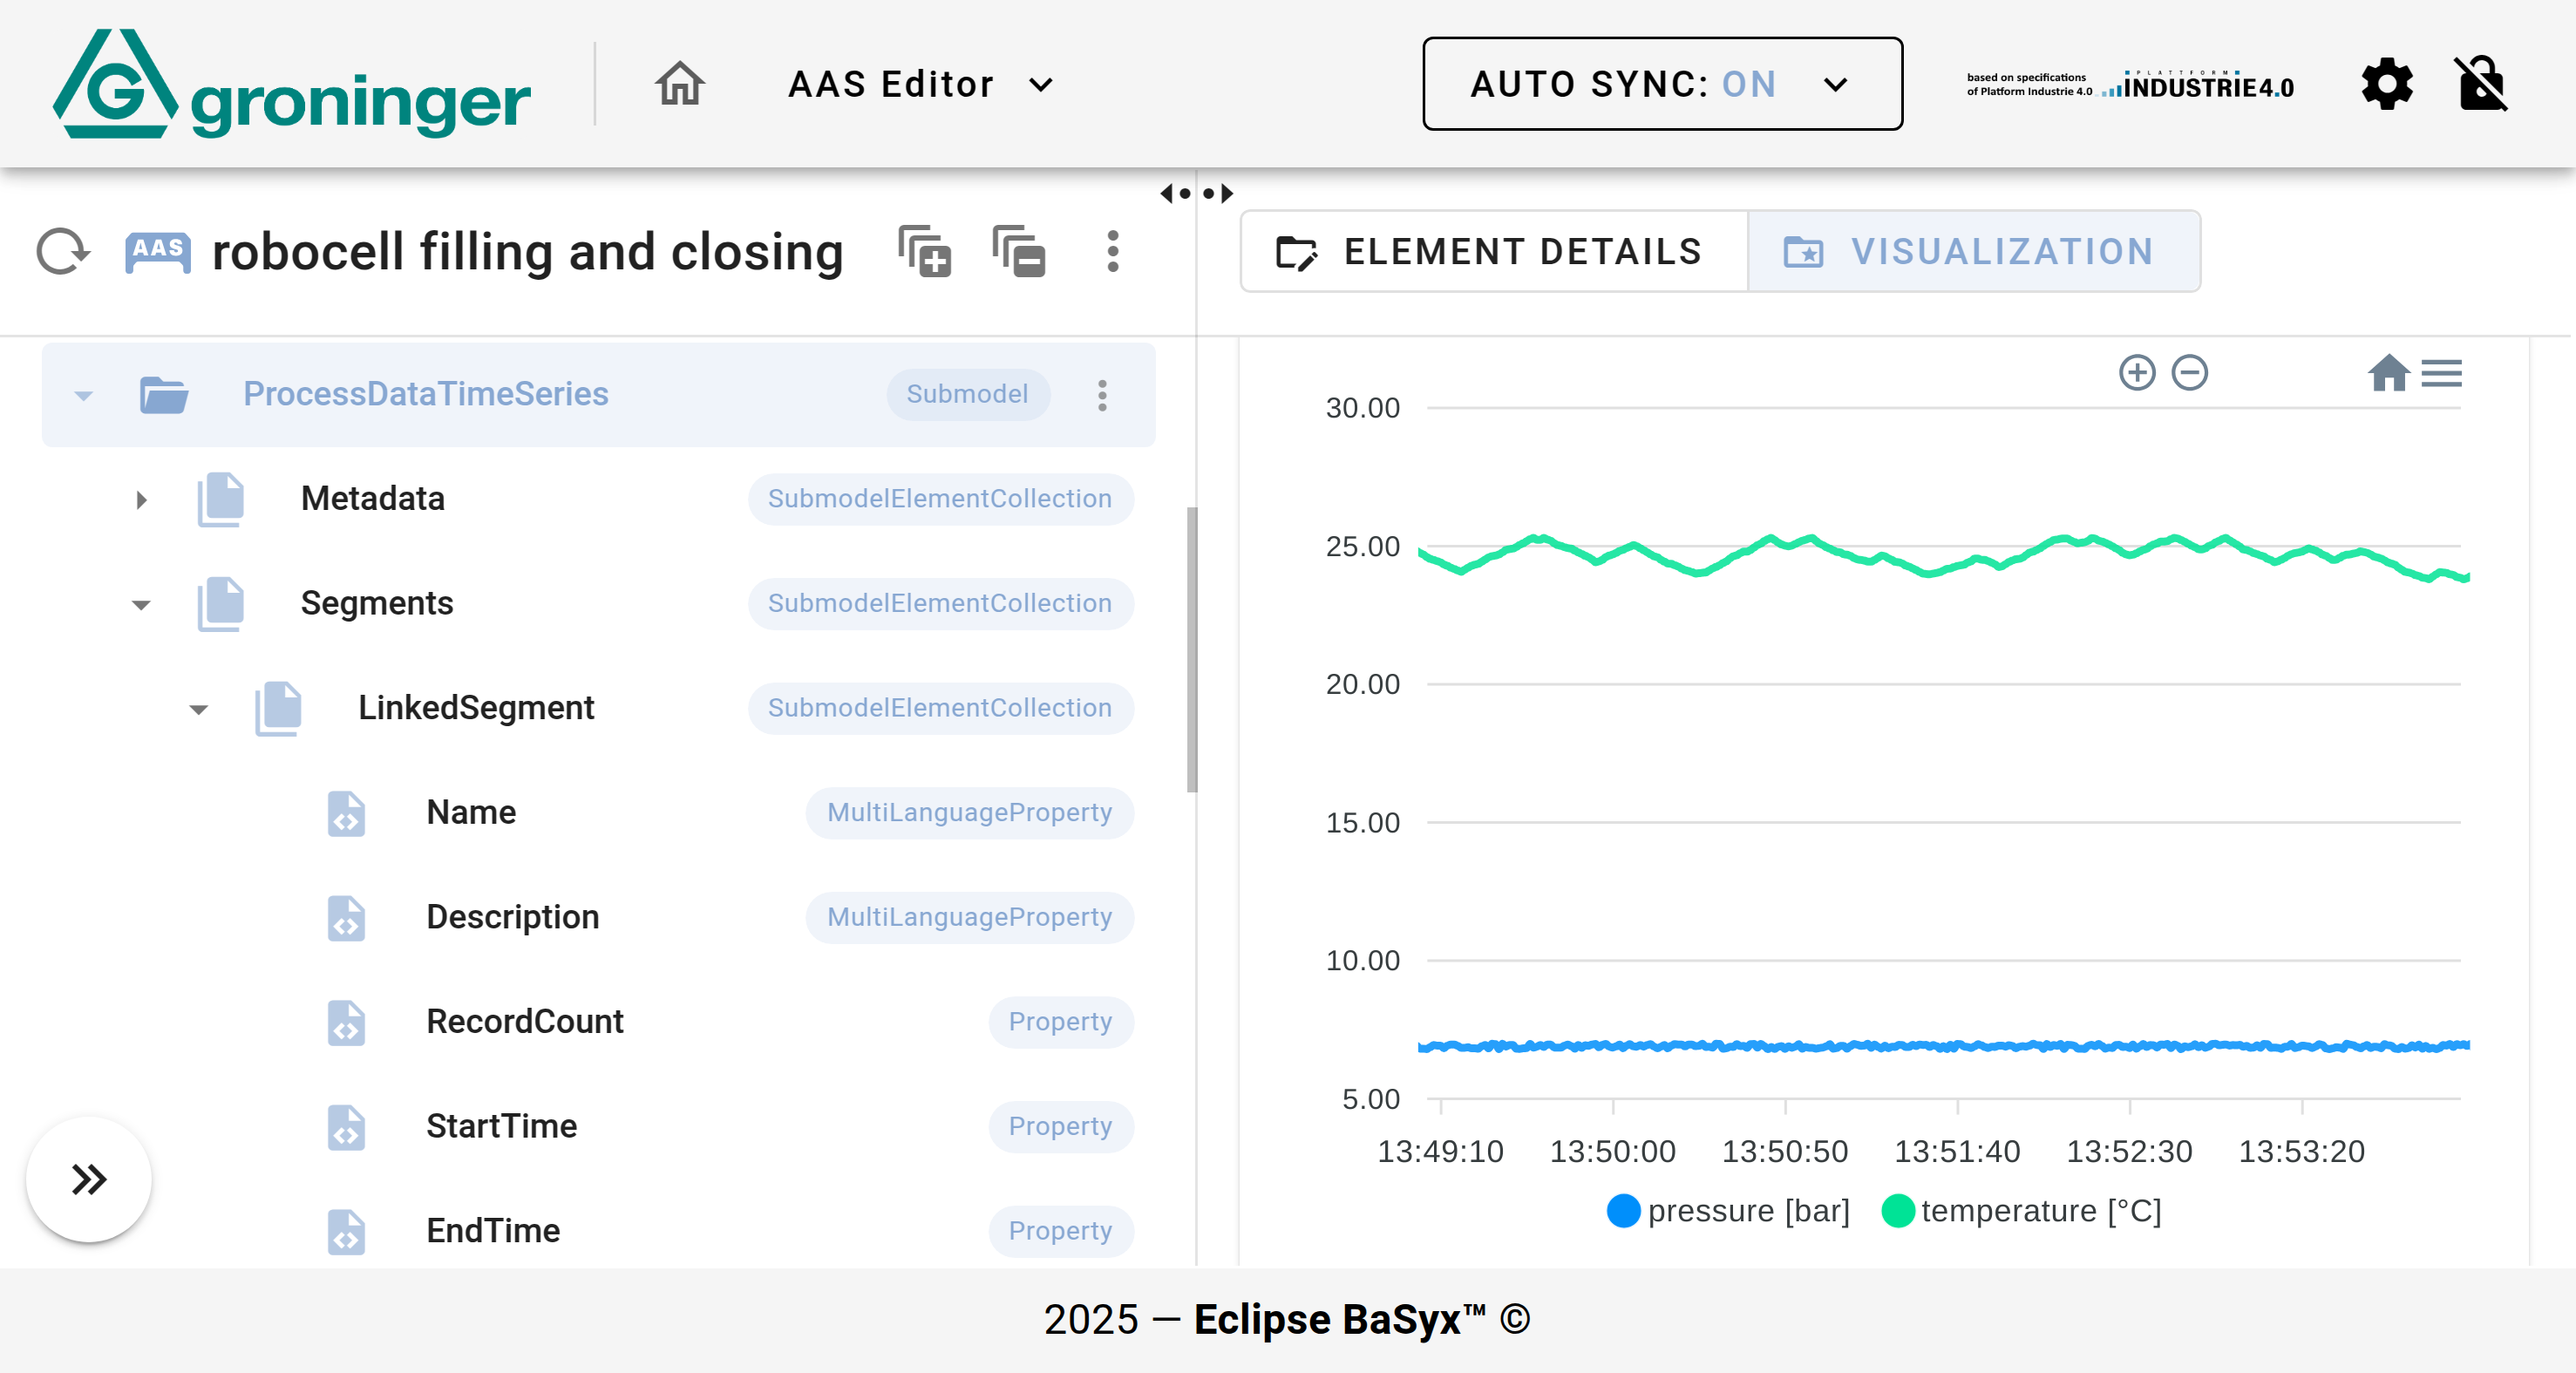
\includegraphics[width=1\textwidth]{Bilder/ErgebnisseAASWebUI/Zeitreihen.png}
    \caption[Visualisierung Submodell Zeitreihendaten]{Visualisierung Submodell Zeitreihendaten (Liniendiagramm)}
    \label{fig:LiniendiagrammBaSyx}
\end{figure}
\vspace{-0.5em}

Ein wesentlicher Vorteil dieser Umsetzung liegt in der Entkopplung von Datenspeicherung und \acs{aas}. 
Da die \acs{aas} selbst nicht für die Ablage großer oder historischer Datenmengen ausgelegt ist, ermöglicht die Auslagerung in eine externe Zeitreihendatenbank eine effiziente Speicherung und Verarbeitung. 
Zudem können die Daten durch die strukturierte Referenzierung über das LinkedSegment einfach in weiteren Anwendungen, wie Analysesystemen oder KI gestützten Verfahren, weiterverwendet werden.

\subsubsection{Herausforderungen bei der Implementierung}
Im Rahmen der Implementierung des Demonstrators traten verschiedene Herausforderungen auf, die sowohl technische als auch methodische Aspekte betrafen. 
Diese ergaben sich unter anderem aus der noch jungen Verbreitung der \acs{aas} im Maschinenbau, der eingeschränkten Datenverfügbarkeit sowie den Limitierungen der eingesetzten Werkzeuge. 
Die wesentlichen Punkte sind im Folgenden zusammengefasst:

\begin{enumerate}
    \item \textbf{Fehlende praxisnahe Vorlagen für den Maschinenbau:}  
    Zwar existieren bereits diverse \acsp{smt}, Spezifikationen sowie allgemeine Anwendungsfälle, diese sind jedoch primär auf Komponentenhersteller ausgerichtet.  
    Konkrete Vorlagen und praxisnahe Anwendungsfälle, die speziell auf den Maschinenbau und die Anforderungen des Demonstrators zugeschnitten sind, standen jedoch nur begrenzt zur Verfügung.

    \item \textbf{Begrenzte Datenverfügbarkeit:}  
    Da keine reale Maschine angebunden war, mussten Echtzeitdaten simuliert werden.  
    Zudem waren nicht alle relevanten Daten im PLM-System so dokumentiert, dass eine direkte Übernahme möglich gewesen wäre.  
    Viele Informationen mussten daher manuell aus verschiedenen Dokumenten, wie der Betriebsanleitung, extrahiert werden.  

    \item \textbf{Begrenzte Verfügbarkeit semantischer Beschreibungen:}  
    Für viele spezifische Maschineneigenschaften, wie technische Parameter im Verarbeitungsbereich (z.\,B. Spritze, Vial, Zylinderampulle) und deren Detailwerte (z.\,B. Füllmenge, Stopfenhöhe), existieren bislang keine standardisierten ECLASS-Beschreibungen.  
    Diese mussten daher manuell angelegt werden, was zeitaufwendig war und die Interoperabilität einschränkt.

    \item \textbf{Eingeschränkte Funktionalität der eingesetzten Tools:}  
    Die verwendeten Werkzeuge unterstützten nicht alle benötigten Funktionen.  
    So wurden beispielsweise beim Hochladen von Dateien in der AAS Web UI keine Einträge im Discovery Service erzeugt.  
    Da diese Funktionalität erforderlich war, musste sie mithilfe eines eigens entwickelten Skripts ergänzt werden.  
    Eine detailliertere Evaluierung der eingesetzten Tools erfolgt in Kapitel \ref{subsec:EvaluierungTools}.

    \item \textbf{Inkonsistenzen zwischen Spezifikationen und Tools:}  
    \acsp{smt} und die zugehörigen Spezifikationen wiesen teilweise Inkonsistenzen auf, etwa unterschiedliche Werte in der Dokumentation im Vergleich zu den AASX-Vorlagen.  
    Dies führte dazu, dass einige Plugins nicht oder nur eingeschränkt funktionierten, da sie auf korrekte semantische Beschreibungen angewiesen sind.  
    Die Fehlerbehebung erforderte eine manuelle Anpassung der \acsp{smt}, was zusätzlichen Aufwand verursachte.
\end{enumerate}

\newpage
\subsection{KI-Modell zur Anomalieerkennung}

Für die Anomalieerkennung wurde der zuvor trainierte Autoencoder im Evaluierungsmodus eingesetzt, sodass während der Auswertung keine Anpassungen der Modellparameter erfolgten.
Die Testdaten basieren, wie beim Training, auf simulierten Temperaturverläufen aus dem Datengenerator, die analog zu den Zeitreihendaten in Kapitel \ref{sec:DynamischeSubmodelle} in einer InfluxDB gespeichert wurden.

Als Eingabe erhält das Modell kurze Sequenzen von jeweils fünf Messwerten.
Im Unterschied zur Trainingsphase enthalten die Testdaten gezielt eingefügte Anomalien, um die Erkennungsfähigkeit des Modells zu prüfen.
Dabei wurden vier Anomalietypen simuliert: dauerhaft erhöhte Werte, ein einzelner ausgeprägter Peak, ein linearer Anstieg über mehrere Zeitpunkte sowie invertierte Werte im Vergleich zum Normalverlauf.

Während der Auswertung berechnet der Autoencoder für jede Sequenz den Rekonstruktionsfehler als durchschnittliche Abweichung zwischen Eingabe- und Ausgabedaten. 
Zur Klassifikation dient ein Schwellenwert, der aus dem Mittelwert des Fehlers plus dem Zweifachen der Standardabweichung gebildet wird. 
Überschreitet der Fehler einer Sequenz diesen Wert, wird das gesamte Zeitfenster als Anomalie markiert.

Zur Veranschaulichung werden zwei Beispiele gezeigt, die unterschiedliche Anomalietypen repräsentieren. 
Abbildung~\ref{fig:Fall1} zeigt einen Temperaturverlauf mit dauerhaft erhöhten Werten im Bereich t = 10000 - 10010 (gezielt eingefügte Anomalie). 
Das Modell erkennt die Anomalie zuverlässig, allerdings leicht verzögert. 
Dies liegt an der Mittelwertbildung über das Fünf-Werte-Fenster.
Erst wenn mehrere aufeinanderfolgende Werte vom Normalverlauf abweichen, steigt der Fehler ausreichend an.

\vspace{-0.75em}
\begin{figure}[htbp]
    \centering
        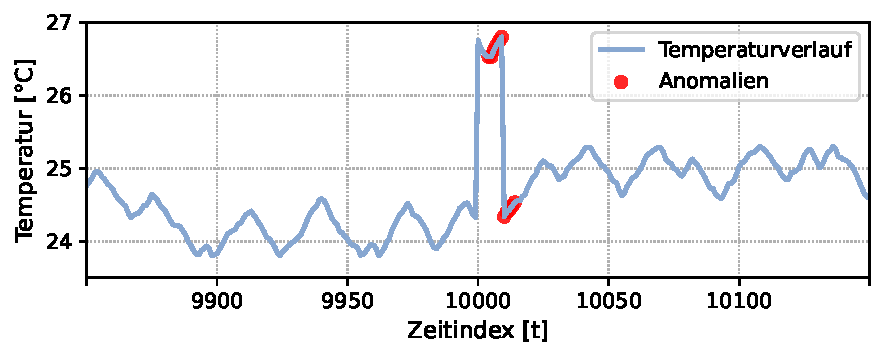
\includegraphics[width=1\textwidth]{Bilder/Ergebnisse/KI/Fall1.pdf}
        \vspace{-2em}
    \caption[Anomalieerkennung - Fall 1]{Anomalieerkennung - Fall 1: Temperaturverlauf mit überhöhten Werten}
    \label{fig:Fall1}
\end{figure}
\vspace{-0.75em}

In Abbildung~\ref{fig:Fall2} ist ein Temperaturverlauf mit einem gleichmäßigen, linearen Anstieg im Bereich t = 25343 - 25393 (gezielt eingefügte Anomalie) dargestellt. 
Auch hier%
\pagebreak
~klassifiziert das Modell den Verlauf korrekt als Anomalie. 
Dies zeigt, dass die Erkennung nicht nur auf plötzliche Ausreißer reagiert, sondern auch schleichende Veränderungen im Signalverlauf erkennt.

\vspace{-0.75em}
\begin{figure}[htbp]
    \centering
        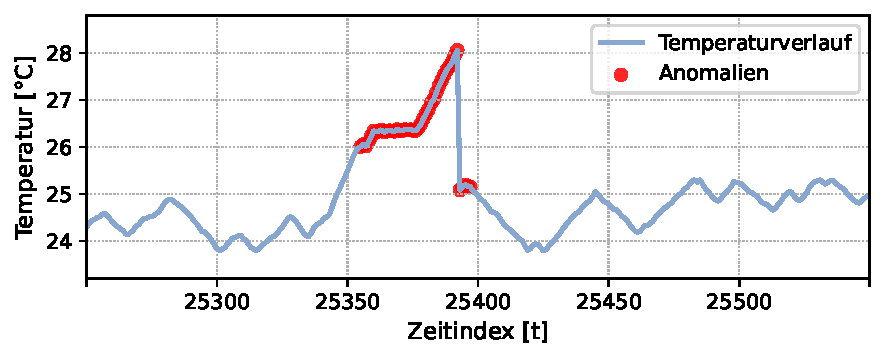
\includegraphics[width=1\textwidth]{Bilder/Ergebnisse/KI/Fall2.pdf}
        \vspace{-2em}
    \caption[Anomalieerkennung - Fall 2]{Anomalieerkennung - Fall 2: Temperaturverlauf mit linearem Anstieg}
    \label{fig:Fall2}
\end{figure}
\vspace{-0.75em}

In allen Testfällen mit künstlich erzeugten Anomalien erfolgte die Klassifikation korrekt, ohne Fehlalarme. 
Aufgrund der Fenstergröße und der Mittelwertbildung tritt die Markierung jedoch häufig leicht verzögert auf, wodurch einzelne Sequenzen innerhalb einer Anomaliephase nicht als abweichend markiert werden. 
Da ausschließlich synthetische Abweichungen geprüft wurden, ist zu erwarten, dass reale Anomalien aufgrund ihrer höheren Komplexität eine größere Herausforderung darstellen.

Zur Verbesserung könnten umfangreichere und variantenreichere Trainings- und Testdaten eingesetzt werden. 
Auch leistungsfähigere Architekturen wie tiefere Autoencoder oder LSTM-basierte Netze (Long Short-Term Memory, eine spezielle Form rekurrenter neuronaler Netze zur Verarbeitung von Zeitreihen) bieten Potenzial, zeitliche Abhängigkeiten präziser zu erfassen \cite{MALEKI2021107443}. 
Diese Ansätze wurden aufgrund begrenzter Rechenressourcen im Rahmen dieser Arbeit jedoch nicht weiterverfolgt, können aber eine Grundlage für zukünftige Entwicklungen bilden.

Dennoch zeigt sich, dass das gewählte Konzept grundsätzlich umsetzbar ist und sich für eine Einbettung in industrielle Szenarien eignet. 
In Verbindung mit realen Maschinendaten könnten erkannte Anomalien genutzt werden, um proaktive Wartungsmaßnahmen einzuleiten. 
Dadurch ließe sich die Anlagenverfügbarkeit erhöhen und ungeplante Stillstandszeiten verringern.
Werden neben Sensordaten zusätzlich technische Stammdaten oder standardisierte Beschreibungen berücksichtigt, wie sie auch im AAS-Demonstrator hinterlegt sind, wird eine noch umfassendere Analyse möglich, die zugleich die Grundlage für weiterführende \acs{pm}-Ansätze bilden könnte.

\newpage
\subsection{Anwendungsfall Digitaler Produktpass}
% Der Anwendungsfall \acs{dpp} demonstriert, wie Nachhaltigkeitsinformationen in Form von \acs{pcf}-Werten direkt in der AAS einer Maschine abgebildet und anschließend nutzer- bzw. rollenabhängig bereitgestellt werden können. 
% Grundlage bildet der in Kapitel \ref{sec:AAS-Demonstrator} vorgestellte AAS-Demonstrator, der um ein Submodell zur Abbildung des \acs{cf} erweitert wurde. 
% Neben der dynamischen Berechnung und Aggregation dieser Werte wird daher auch gezeigt, wie der Zugriff auf die im DPP enthaltenen Informationen durch unterschiedliche Nutzerrollen und technische Clients geregelt ist.

Mit dem Anwendungsfall \acs{dpp} konnte gezeigt werden, dass Nachhaltigkeitsinformationen in Form von \acs{pcf}-Werten direkt in der AAS einer Maschine abgebildet und nutzer- bzw. rollenabhängig bereitgestellt werden können.
Im Folgenden wird hierzu sowohl die Aggregation der Werte als auch die Umsetzung des rollenbasierten Zugriffs durch unterschiedliche Nutzerrollen und technische Clients dargestellt.
Grundlage bildet der in Kapitel~\ref{sec:AAS-Demonstrator} vorgestellte AAS-Demonstrator, der um ein Submodell zur Abbildung des \acs{cf} erweitert wurde.

\subsubsection{Abbildung des PCF}
Das CF-Submodell bildet die Lebenszyklusphasen Material, Produktion und Cradle to Gate jeweils in eigenen \acsp{smc} ab.
Abbildung~\ref{fig:SubmodellCF} zeigt exemplarisch die \acs{smc} für die Phase Cradle to Gate (links) sowie die integrierte Komponentenliste (rechts), in der die für die Berechnung herangezogenen Siemens-Komponenten hinterlegt sind.

\begin{figure}[htbp]
    \centering
        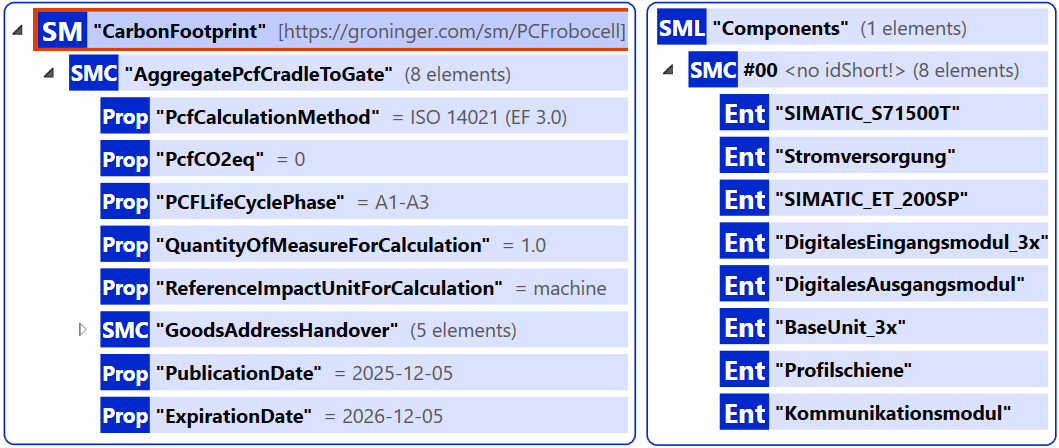
\includegraphics[width=1\textwidth]{Bilder/ErgebnissePackageExplorer/CarbonFoorprintTest.png}
    \caption{Ausschnitt Submodell \acs{cf}}
    \label{fig:SubmodellCF}
\end{figure}
\vspace{-0.5em}

Die Aggregation der CO\textsubscript{2}-Äquivalente erfolgt dynamisch über einen Microservice. 
Dieser ist als Docker-Container implementiert und greift über die REST-Schnittstellen des BaSyx-Backends auf die in der Komponentenliste hinterlegten Entitäten zu. 
Mithilfe des Discovery Service werden deren AAS identifiziert und vorhandene CF-Submodelle ausgelesen. 
Die enthaltenen PCF-Werte werden anschließend zu Gesamtwerten für die einzelnen Lebenszyklusphasen aggregiert und in das CF-Submodell der Haupt-AAS zurückgeschrieben.

Die Berechnung kann direkt über ein Plugin in der AAS Web UI ausgelöst werden.
Nach Abschluss des Berechnungsprozesses werden die aktualisierten Werte automatisch vom Submodel Repository abgefragt und in der Benutzeroberfläche aktualisiert.
Abbildung~\ref{fig:PluginAggregation} zeigt die entsprechende Visualisierung: links die aggregierten CO\textsubscript{2}-Äquivalente, rechts die zugehörigen Lebenszyklusphasen.

\begin{figure}[htbp]
    \centering
        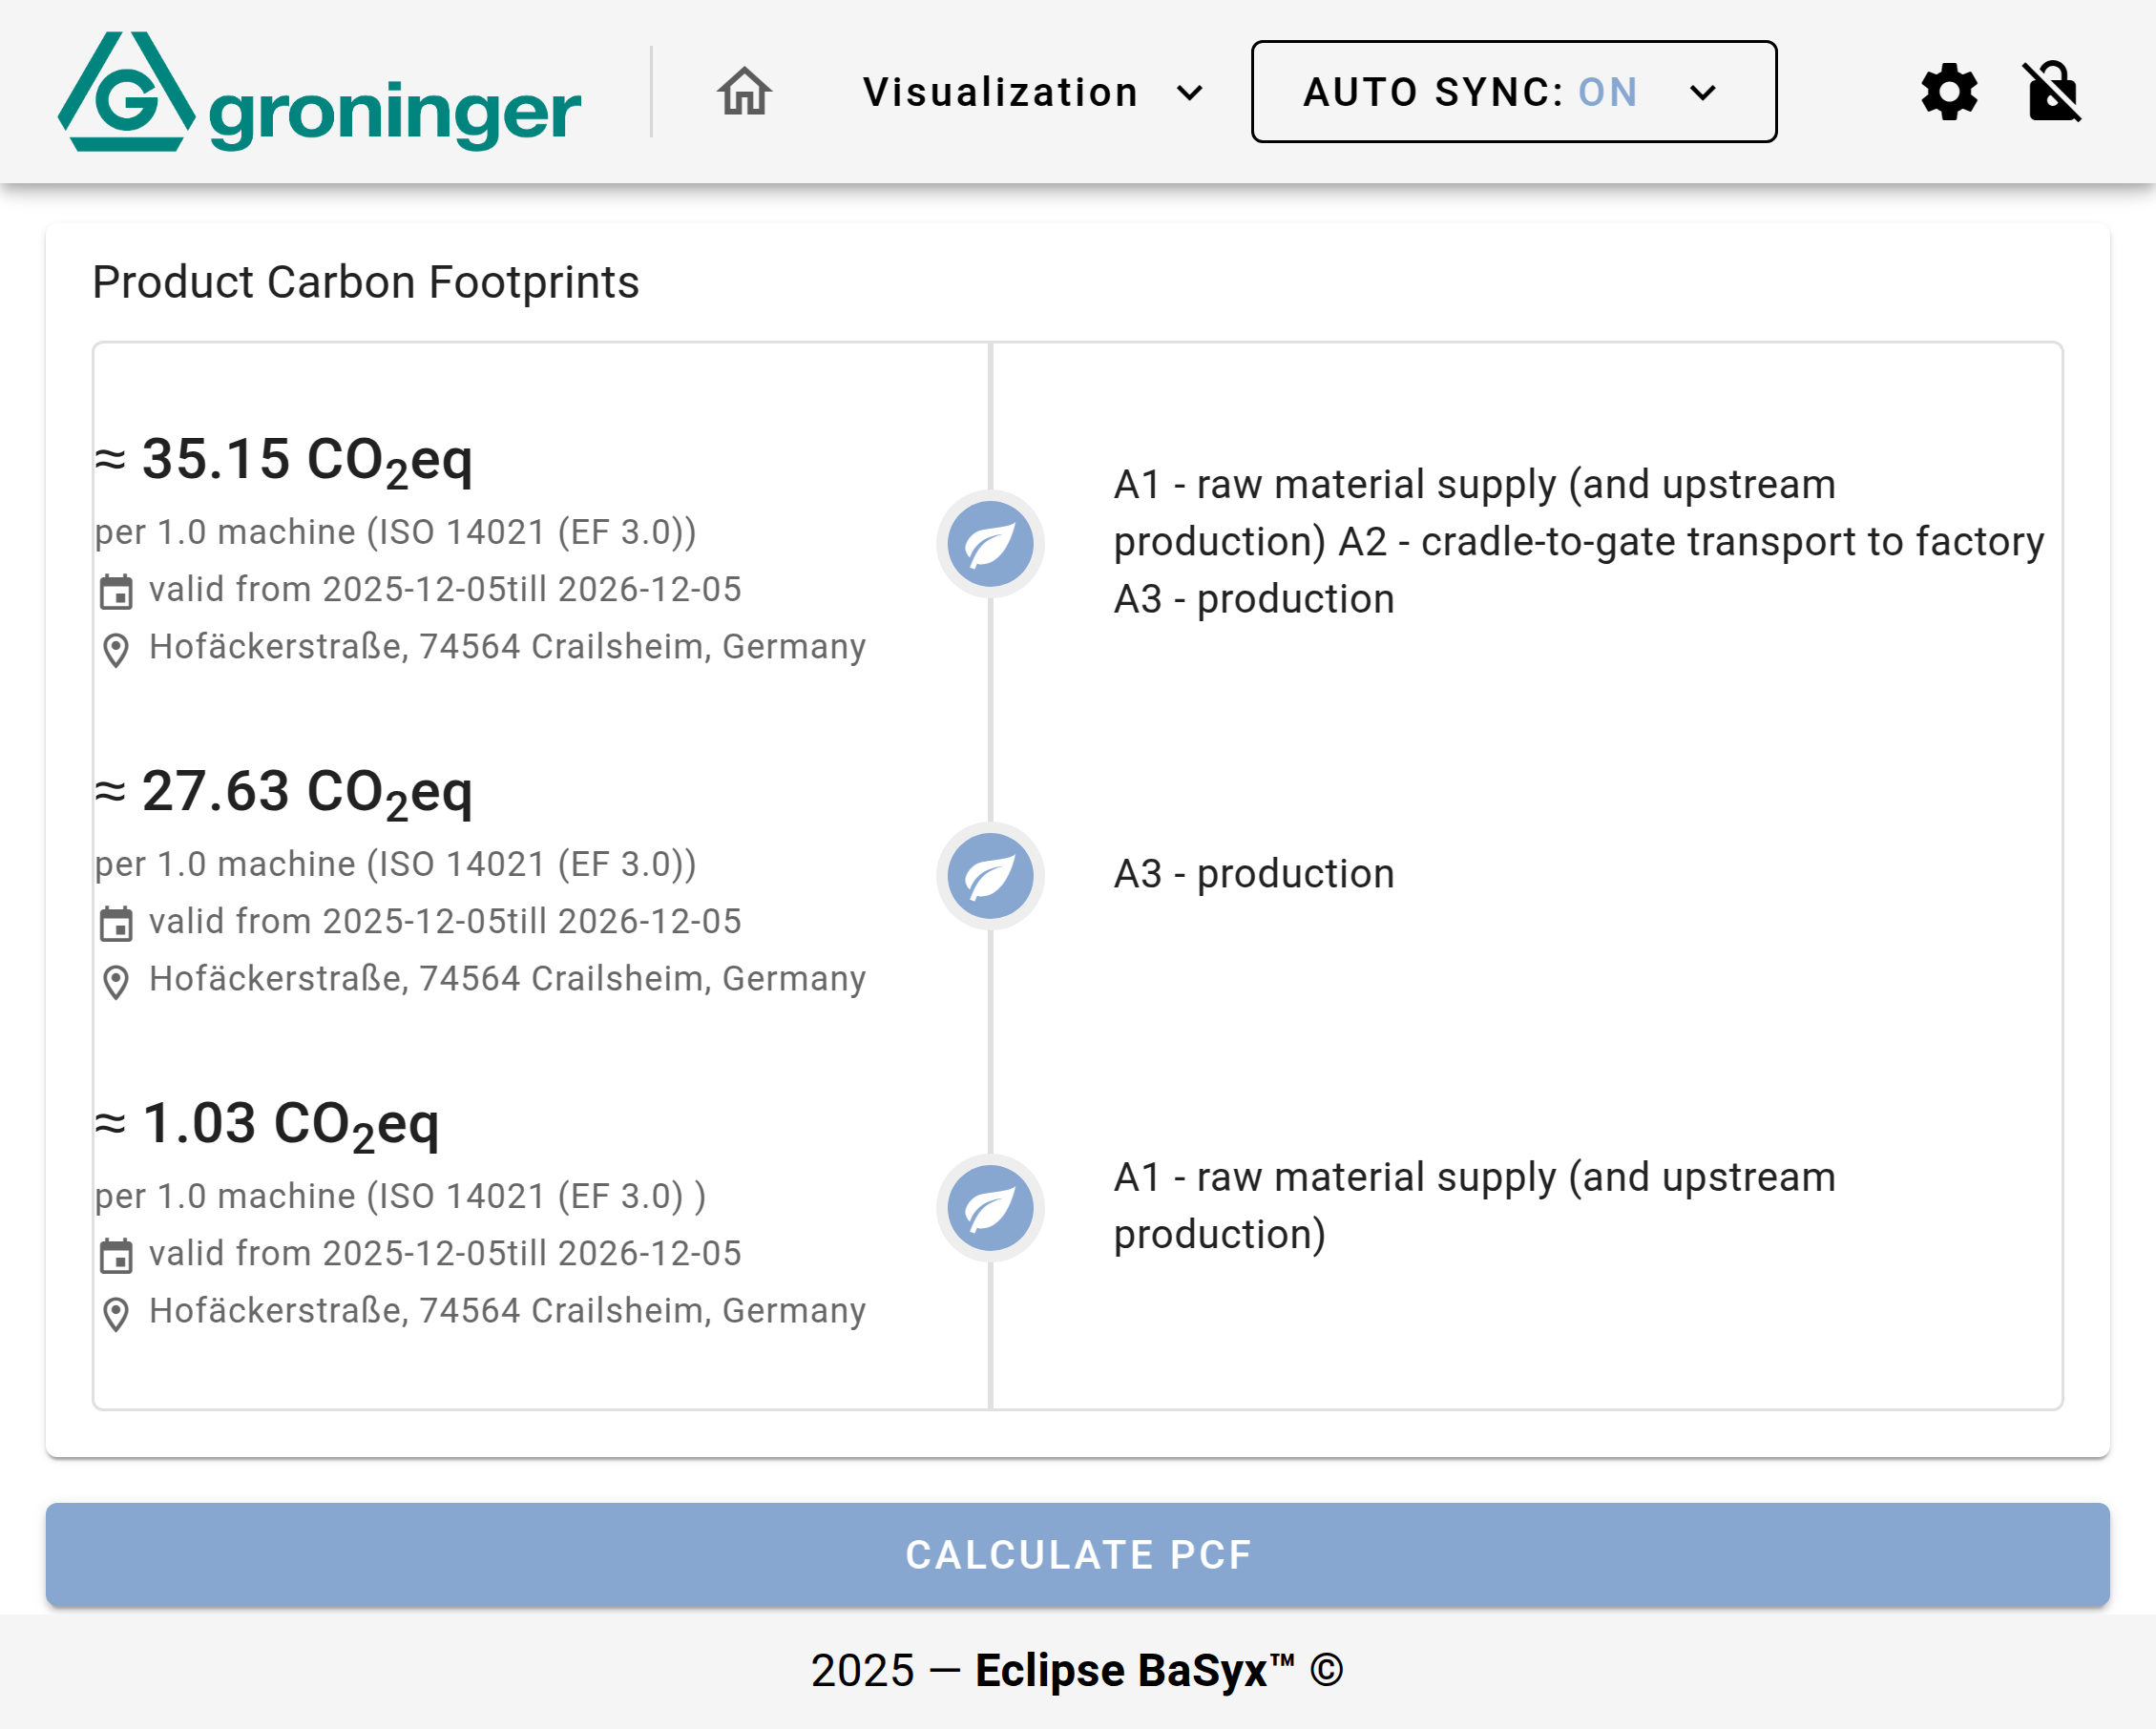
\includegraphics[width=1\textwidth]{Bilder/ErgebnisseAASWebUI/CarbonFootprint.png}
    \caption{Visualisierung \acs{pcf}-Werte je Lebenszyklusphase}
    \label{fig:PluginAggregation}
\end{figure}
\vspace{-0.5em}

Der Ansatz ist flexibel erweiterbar.
Bei Verfügbarkeit weiterer Komponenten-AAS lässt sich die Liste unkompliziert ergänzen, sodass sukzessive die gesamte Maschine berücksichtigt werden kann. 
Perspektivisch ist auch eine Erweiterung auf weitere Lebenszyklusphasen, wie Nutzung oder Entsorgung, sowie die Einbeziehung des TCF denkbar, um eine ganzheitliche ökologische Bilanzierung zu ermöglichen.

Auf diese Weise wird nicht nur die Transparenz gestärkt, sondern auch die Rückverfolgbarkeit, da die einzelnen Beiträge durch die Einbindung separater Komponenten-AAS eindeutig zuordenbar sind. 
Insgesamt verdeutlicht die Umsetzung, dass sich mit der AAS ein \acs{dpp} realisieren lässt, der auch nachhaltigkeitsbezogene Daten standardisiert abbildet und entlang der Wertschöpfungskette nachvollziehbar zur Verfügung gestellt werden kann.

\newpage
\subsubsection{Rollenbasierter Zugriff auf Submodelle}
Der \acs{dpp} wird durch die zuvor erweiterte \acs{aas} des Abfüll- und Verschließmoduls repräsentiert. 
Um sensible Inhalte gezielt und sicher bereitzustellen, wurde eine rollenbasierte Zugriffskontrolle implementiert. 
Die Authentifizierung und Autorisierung erfolgt über Keycloak, das als Docker-Container in die BaSyx-Architektur integriert ist.

Zur Veranschaulichung wurden drei Nutzer mit typischen Rollen eingerichtet, deren zugehörige Berechtigungen in Tabelle~\ref{tab:RBACUsers} dokumentiert sind.

{\small
\begin{longtblr}[
  label = {tab:RBACUsers},
  caption = {Exemplarische Nutzerrollen und zugehörige Berechtigungen im RBAC-Szenario},
  entry = {Nutzerrollen und Berechtigungen im RBAC-Szenario}
]{
  colspec = {l l X[m]}, % dritte Spalte: X[m] = Fließtext, vertikal mittig
  rowhead = 1,
  vlines,
  hlines,
  row{1} = {bg=tableHeader}
}
\textbf{Benutzer} & \textbf{Rolle} & \textbf{Berechtigungen} \\
groninger.meyer & Groninger-Mitarbeiter & Uneingeschränkter Zugriff auf alle Submodelle \\
customer.doe & Kunde & Zugriff auf ausgewählte Submodelle (z.\,B. Typenschild, CF) \\
technician.john & Service-Techniker & Lese- und Schreibrechte auf wartungsrelevante Submodelle \\
\end{longtblr}
}


    
\vspace{-0.25em}
Eine Möglichkeit zur Einsicht der im \acs{dpp} enthaltenen Informationen bietet die AAS Web UI.
Ist \acs{rbac} aktiviert, wird der Benutzer beim Aufruf der Oberfläche automatisch zur Keycloak-Anmeldeseite weitergeleitet.
Wie in Abbildung~\ref{fig:KeycloakAnmeldeSeite} dargestellt, erfolgt die Authentifizierung über die in Keycloak hinterlegten Zugangsdaten.

\vspace{0.4em}
\begin{figure}[htbp]
    \centering
        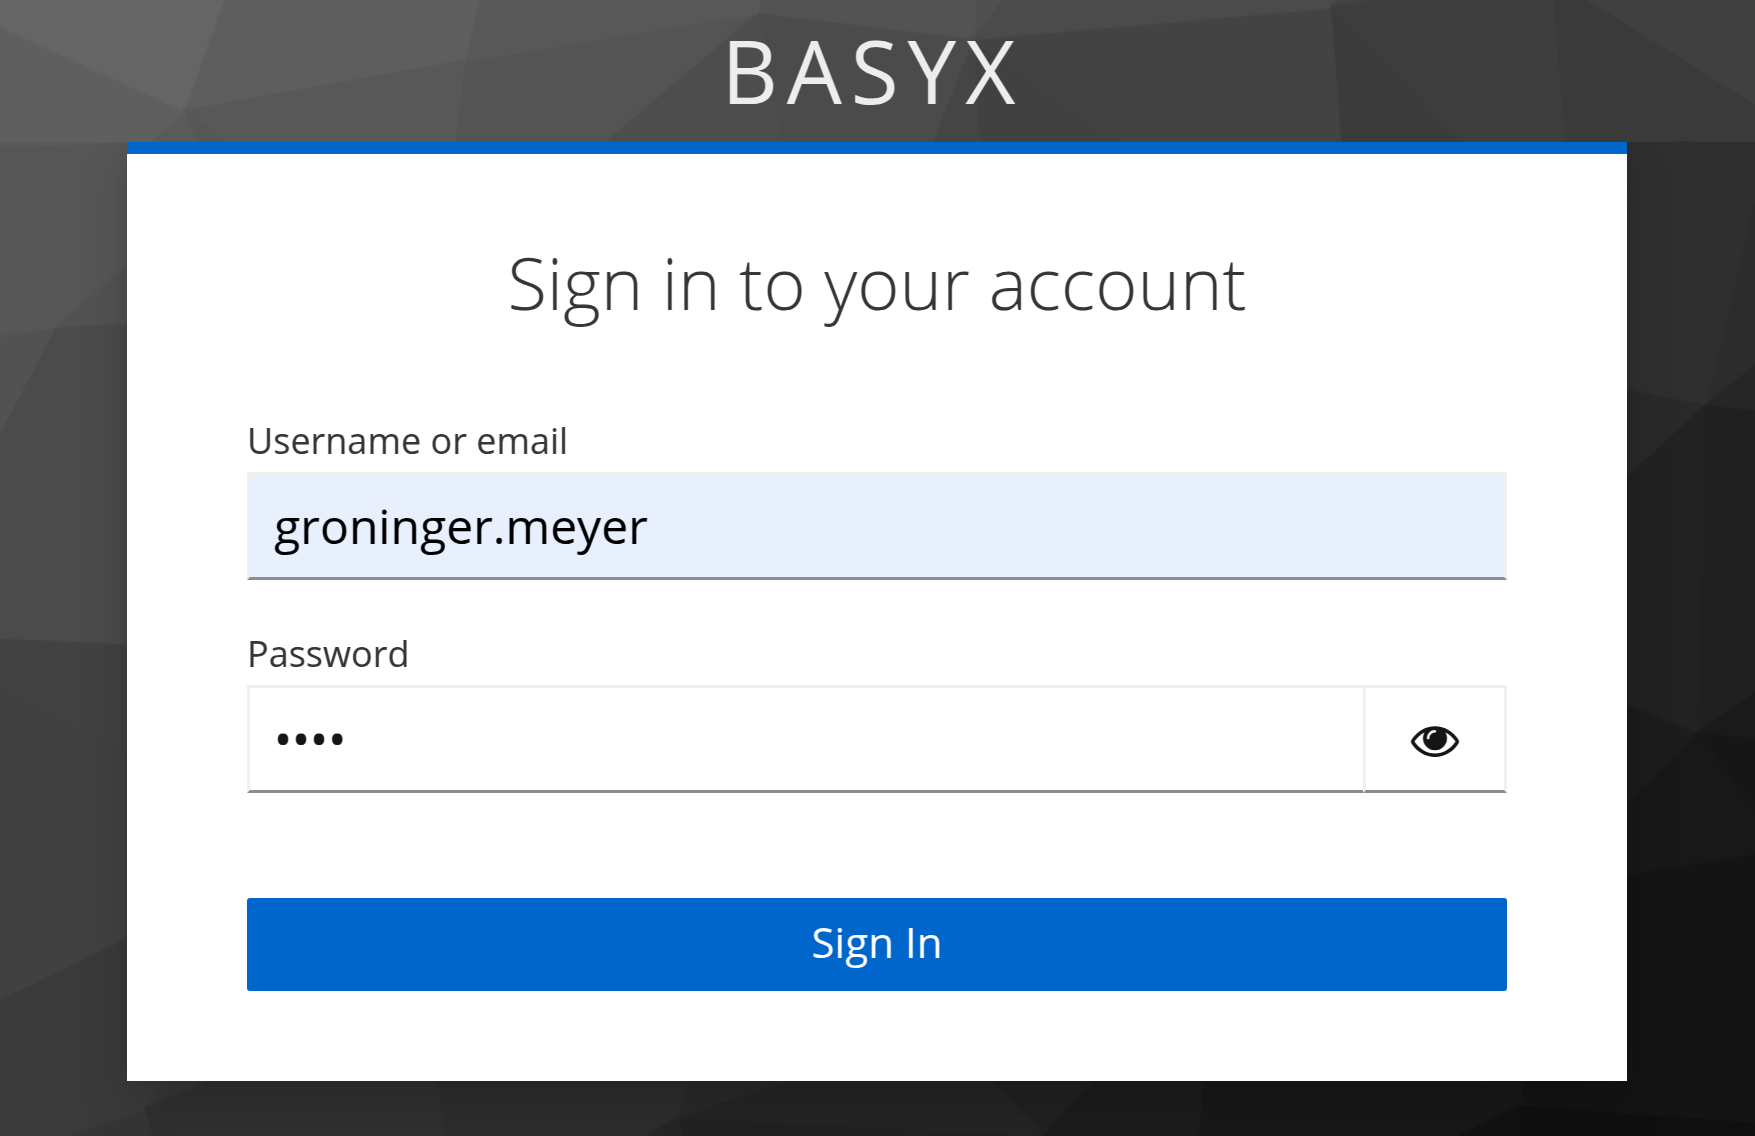
\includegraphics[width=0.7\textwidth]{Bilder/KeycloakAnmeldeSeite.png}
    \caption{Keycloak-Anmeldeseite der AAS Web UI}
    \label{fig:KeycloakAnmeldeSeite}
\end{figure}

\vspace{-0.35em}

Nach erfolgreicher Anmeldung erhält die AAS Web UI ein Zugriffstoken mit den Rolleninformationen, das bei allen weiteren Anfragen an die BaSyx-Komponenten%
\pagebreak
~automatisch mitgesendet wird.
Die jeweiligen Dienste prüfen es gegen die hinterlegten \acs{rbac}-Regeln und entscheiden so über die tatsächliche Zugriffsberechtigung.
Meldet sich etwa customer.doe an, sieht er nur die für seine Rolle freigegebenen Submodelle, während andere verborgen bleiben.
Zudem besitzt er ausschließlich Leserechte, sodass Änderungsversuche mit einem Fehler abgelehnt werden.

Neben der AAS Web UI ist auch ein direkter Zugriff auf die BaSyx-Komponenten über die REST-API möglich, der insbesondere für technische Clients relevant ist. 
Dafür wurden in Keycloak drei Clients mit Service Accounts angelegt, die denselben Rollen wie die Benutzerkonten entsprechen und somit identische Berechtigungen besitzen.

Zur Validierung der Konfiguration wurde Postman eingesetzt. 
Die Clients rufen dabei über den Token-Endpunkt von Keycloak Zugriffstokens ab und nutzen diese für API-Anfragen. 
Abbildung~\ref{fig:DELETEServiceTechniker} zeigt exemplarisch eine DELETE-Anfrage des Service-Techniker-Clients. 
Da dieser nur Leserechte besitzt, wird die Anfrage mit HTTP 403 Forbidden abgelehnt. 
Mit dem Groninger-Client hingegen gelingt der Löschvorgang, da dessen Rolle uneingeschränkte Rechte umfasst.

\begin{figure}[htbp]
    \centering
        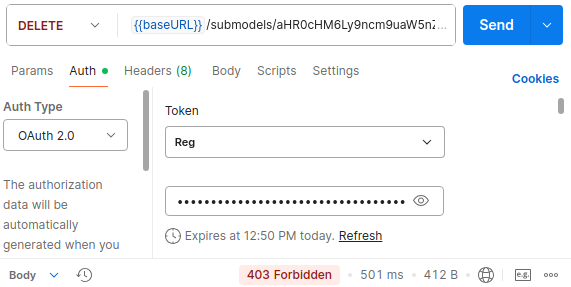
\includegraphics[width=0.95\textwidth]{Bilder/Ergebnisse/DPP/Postman/TechnicianDelet.png}
    \caption[DELETE-Anfrage eines Service-Techniker-Clients]{DELETE-Anfrage eines Service-Techniker-Clients (Postman)}
    \label{fig:DELETEServiceTechniker}
\end{figure}
\vspace{-0.25em}

Die Zugriffskontrolle mit BaSyx und Keycloak zeigt, dass sich Berechtigungen zuverlässig auf die AAS und ihre Submodelle übertragen lassen. 
Dies bestätigt die Eignung der AAS als technische Grundlage für den \acs{dpp} und eröffnet Potenziale für Szenarien, in denen sensible Informationen, etwa Nachhaltigkeitsdaten, differenziert entlang der Wertschöpfungskette bereitgestellt werden. 
Gleichzeitig bleibt der \acs{rbac}-Ansatz in seiner Flexibilität begrenzt, sodass für komplexe Szenarien eine attributbasierte Zugriffskontrolle (\acs{abac}) erforderlich ist, die von BaSyx bislang jedoch nicht unterstützt wird.

\newpage
\subsection{Anwendungsfall automatisierte Generierung von AAS}

Der Anwendungsfall der automatisierten Generierung zeigt, wie sich \acs{aas}-Instanzen automatisch erzeugen und in das BaSyx-Backend integrieren lassen.
Abbildung~\ref{fig:AutomatisierteGenerierungAblauf} veranschaulicht den Ablauf.
Ausgangspunkt bildet ein unternehmensspezifisches \acs{smt}, das mithilfe des Package Explorers aus dem generischen SMT Generic Frame for Technical Data for Industrial Equipment in Manufacturing \cite{SpezifikaitonTechnischeDaten} abgeleitet wurde.

\begin{figure}[htbp]
    \centering
        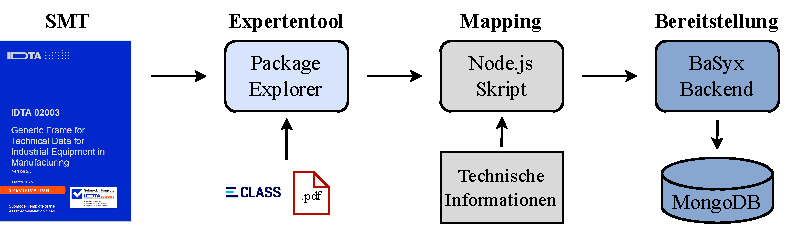
\includegraphics[width=\textwidth]{Bilder/ErgebnisseAutomatisierteGenerierung/ARchitekturTest.pdf}
    \caption[Automatisierte Generierung einer AAS]{Automatisierte Generierung einer AAS (eigene Darstellung; Bildbestandteile: \cite{SpezifikaitonTechnischeDaten}, \cite{ECLASSLogo} )}
    \label{fig:AutomatisierteGenerierungAblauf}
\end{figure}
\vspace{-0.5em}

Das resultierende Typ-Submodell wird durch ein Node.js-basiertes Mapping-Skript mit Beispieldaten angereichert und in eine neue \acs{aas}-Instanz eingebettet. 
Das Skript übernimmt zusätzlich die Registrierung im BaSyx-Backend, sodass die erzeugte \acs{aas} unmittelbar zur Verfügung steht und beispielsweise in der AAS Web UI visualisiert werden kann.

In der prototypischen Umsetzung zeigte sich, dass der entwickelte Ansatz den manuellen Modellierungsaufwand im Package Explorer potenziell erheblich reduzieren kann, insbesondere bei komplexen Submodellstrukturen wäre dies ein großer Vorteil. 
Zudem ist der Prozess grundsätzlich auch auf weitere Submodelle übertragbar, sodass perspektivisch die \acs{aas} einer gesamten Maschine automatisiert generiert werden könnte. 

Im Rahmen dieses Anwendungsfalls wurden zwar statische Beispieldaten verwendet. 
In einer produktiven Umgebung könnten die technischen Produktinformationen jedoch direkt aus bestehenden \acs{it}-Systemen übernommen werden. 
Bei groninger liegen diese Daten überwiegend im \acs{plm}-System Agile vor. 
Eine technische Anbindung ist dort derzeit allerdings nicht möglich und konnte in dieser Arbeit nicht realisiert werden.

Darüber hinaus ließe sich die Mapping-Logik in eine Laufzeitumgebung integrieren, wodurch Generierung, Bereitstellung und Aktualisierung von \acs{aas}-Instanzen vollständig automatisiert erfolgen könnten. 
Damit eröffnet der Ansatz die Möglichkeit, den Aufbau digitaler Zwillinge zukünftig wesentlich effizienter zu gestalten und die Interoperabilität weiter zu erhöhen.

%Evaluation der eingesetzten Software
\newpage
\subsection{Evaluierung eingesetzter Tools und Software}
\label{subsec:EvaluierungTools}
Zur Umsetzung des AAS-Demonstrators sowie der zugehörigen Anwendungsfälle kamen zwei zentrale Softwarelösungen zum Einsatz.
Im Folgenden werden diese mit Blick auf ihre Funktionalität sowie ihre Stärken und Schwächen evaluiert.
Die Bewertung stützt sich dabei auf die Erfahrungen aus der praktischen Anwendung und berücksichtigt sowohl technische Aspekte als auch die Benutzerfreundlichkeit.

\subsubsection{Package Explorer}

Der Package Explorer wurde während der gesamten Projektlaufzeit als zentrales Modellierungstool eingesetzt.
Er ermöglichte die Erstellung, Bearbeitung und Visualisierung von AAS einschließlich ihrer Submodelle und Submodellelemente.
Besonders hilfreich war die Möglichkeit, semantische Beschreibungen direkt aus ECLASS-Katalogen zu importieren.
Dadurch verringerte sich der ansonsten sehr aufwendige manuelle Aufbau eigener Concept Descriptions deutlich, was den Modellierungsprozess spürbar beschleunigte.
Zudem überzeugte die benutzerfreundliche Oberfläche, die den Einstieg erleichterte, das Verständnis der AAS-Strukturen förderte und Verstöße gegen die Spezifikation der IDTA unmittelbar kenntlich machte.

In der praktischen Anwendung zeigten sich jedoch auch Einschränkungen.
Die integrierte Validierungsfunktion erwies sich als unzuverlässig, sodass zur Absicherung eine separate Test-Engine erforderlich war.
Während die Anbindung an den AASX Server Blazor problemlos funktionierte, war eine direkte Integration in modulare Laufzeitsysteme wie Eclipse BaSyx nicht möglich.
Die AAS mussten daher manuell bereitgestellt werden, was insbesondere bei einer größeren Anzahl oder häufigen Änderungen mit erheblichem Mehraufwand verbunden war.
Darüber hinaus wich der Package Explorer in einzelnen Punkten von den aktuellen AAS-Spezifikationen ab, was vereinzelt zu fehlerhaften semantischen Angaben führte, die nachträglich korrigiert werden mussten.

Insgesamt erwies sich der Package Explorer als hilfreiches Werkzeug für die statische Modellierung von Typ-1-\acs{aas}.
Die vorhandenen Exportfunktionen, insbesondere im AASX-Format, erleichterten die Weiterverwendung und Weitergabe maßgeblich.
Für automatisierte Szenarien bot das Tool hingegen nur eingeschränkte Unterstützung, die sich im Wesentlichen auf das Anlegen eigener \acsp{smt} beschränkte.

\newpage
\subsubsection{Eclipse BaSyx}

Die Eclipse-BaSyx-Plattform bildete in diesem Projekt die zentrale Laufzeitumgebung für den Betrieb von \acs{aas}.
Ein wesentlicher Vorteil war der modulare Aufbau, der praxisnahe Szenarien und zugleich eine flexible Konfiguration ermöglichte.
%der die Umsetzung praxisnaher Industrieszenarien erlaubte und zugleich eine flexible Konfiguration einzelner Komponenten zuließ.
Ebenso eröffneten die standardisierten REST-APIs einen direkten Zugriff auf die einzelnen Komponenten, der dank der integrierten Swagger-Dokumentation unmittelbar getestet und transparent nachvollzogen werden konnte.
Darüber hinaus erleichterte die DataBridge die Anbindung unterschiedlicher Protokolle, insbesondere von \acs{opcua}, wodurch eine dynamische Erweiterung der AAS und die Umsetzung dynamischer Submodelle möglich wurde.

Mit der AAS Web UI stand zudem eine Benutzeroberfläche zur Verfügung, die sowohl die Darstellung als auch die Anpassung von AAS erlaubte. 
Für zentrale Submodelle existieren bereits spezialisierte Plugins, die sich aufgrund des Open-Source-Charakters einfach erweitern oder ergänzen ließen.
% So konnten weitere Submodelle integriert und projektspezifische Anforderungen berücksichtigt werden.
Als besonders hilfreich erwies sich zudem die Synchronisationsfunktion, die insbesondere in dynamischen Szenarien sicherstellte, dass die angezeigten Daten stets aktuell blieben.

Aufgrund der Komplexität des Gesamtsystems war jedoch ein erheblicher Konfigurationsaufwand erforderlich.
Dies betraf nicht nur die initiale Einrichtung, sondern zeigte sich auch bei der Konfiguration der rollenbasierten Zugriffskontrolle (\acs{rbac}), die für jede Komponente separat vorgenommen werden musste.
Hinzu kam, dass der Start des Systems in der Docker-Umgebung vergleichsweise lange dauerte (bis zu mehreren Minuten).
Dies erwies sich insbesondere bei häufigen Anpassungen oder Testläufen als hinderlich.

Darüber hinaus zeigte sich, dass die Plattform in einzelnen Bereichen noch nicht vollständig ausgereift ist.
So war es beispielsweise beim Ändern von Werten innerhalb einer Property über die REST-API nur möglich, String-Werte einzutragen, auch wenn ein anderer Datentyp, wie etwa ein Integer, vorgesehen war.
Zudem erfolgte beim Ablegen aktualisierter \acs{aas} in das gemountete Volume der AAS Environment nicht immer eine zuverlässige Synchronisierung der zugehörigen Concept Descriptions.
In diesen Fällen war ein Start des Gesamtsystems nicht möglich, sodass die betreffenden Einträge in der angebundenen MongoDB gelöscht und anschließend mithilfe eines Skripts nachgeführt werden mussten.

Insgesamt erwies sich Eclipse BaSyx als leistungsfähige Plattform, die bereits für Typ-2-\acs{aas} geeignet ist und perspektivisch auch als Grundlage für Typ-3-\acs{aas} dienen kann.
Der praktische Einsatz zeigte jedoch auch, dass einzelne Funktionalitäten fehlerhaft oder nicht vollständig implementiert sind.
Aufgrund der offenen Architektur können diese zwar korrigiert oder ergänzt werden, erfordern allerdings zusätzlichen Entwicklungsaufwand.









